% Options for packages loaded elsewhere
\PassOptionsToPackage{unicode}{hyperref}
\PassOptionsToPackage{hyphens}{url}
%
\documentclass[
]{article}
\title{Nuclear Energy: Kahan scale and Economic Political value scale}
\author{}
\date{\vspace{-2.5em}}

\usepackage{amsmath,amssymb}
\usepackage{lmodern}
\usepackage{iftex}
\ifPDFTeX
  \usepackage[T1]{fontenc}
  \usepackage[utf8]{inputenc}
  \usepackage{textcomp} % provide euro and other symbols
\else % if luatex or xetex
  \usepackage{unicode-math}
  \defaultfontfeatures{Scale=MatchLowercase}
  \defaultfontfeatures[\rmfamily]{Ligatures=TeX,Scale=1}
\fi
% Use upquote if available, for straight quotes in verbatim environments
\IfFileExists{upquote.sty}{\usepackage{upquote}}{}
\IfFileExists{microtype.sty}{% use microtype if available
  \usepackage[]{microtype}
  \UseMicrotypeSet[protrusion]{basicmath} % disable protrusion for tt fonts
}{}
\makeatletter
\@ifundefined{KOMAClassName}{% if non-KOMA class
  \IfFileExists{parskip.sty}{%
    \usepackage{parskip}
  }{% else
    \setlength{\parindent}{0pt}
    \setlength{\parskip}{6pt plus 2pt minus 1pt}}
}{% if KOMA class
  \KOMAoptions{parskip=half}}
\makeatother
\usepackage{xcolor}
\IfFileExists{xurl.sty}{\usepackage{xurl}}{} % add URL line breaks if available
\IfFileExists{bookmark.sty}{\usepackage{bookmark}}{\usepackage{hyperref}}
\hypersetup{
  pdftitle={Nuclear Energy: Kahan scale and Economic Political value scale},
  hidelinks,
  pdfcreator={LaTeX via pandoc}}
\urlstyle{same} % disable monospaced font for URLs
\usepackage[margin=1in]{geometry}
\usepackage{color}
\usepackage{fancyvrb}
\newcommand{\VerbBar}{|}
\newcommand{\VERB}{\Verb[commandchars=\\\{\}]}
\DefineVerbatimEnvironment{Highlighting}{Verbatim}{commandchars=\\\{\}}
% Add ',fontsize=\small' for more characters per line
\usepackage{framed}
\definecolor{shadecolor}{RGB}{248,248,248}
\newenvironment{Shaded}{\begin{snugshade}}{\end{snugshade}}
\newcommand{\AlertTok}[1]{\textcolor[rgb]{0.94,0.16,0.16}{#1}}
\newcommand{\AnnotationTok}[1]{\textcolor[rgb]{0.56,0.35,0.01}{\textbf{\textit{#1}}}}
\newcommand{\AttributeTok}[1]{\textcolor[rgb]{0.77,0.63,0.00}{#1}}
\newcommand{\BaseNTok}[1]{\textcolor[rgb]{0.00,0.00,0.81}{#1}}
\newcommand{\BuiltInTok}[1]{#1}
\newcommand{\CharTok}[1]{\textcolor[rgb]{0.31,0.60,0.02}{#1}}
\newcommand{\CommentTok}[1]{\textcolor[rgb]{0.56,0.35,0.01}{\textit{#1}}}
\newcommand{\CommentVarTok}[1]{\textcolor[rgb]{0.56,0.35,0.01}{\textbf{\textit{#1}}}}
\newcommand{\ConstantTok}[1]{\textcolor[rgb]{0.00,0.00,0.00}{#1}}
\newcommand{\ControlFlowTok}[1]{\textcolor[rgb]{0.13,0.29,0.53}{\textbf{#1}}}
\newcommand{\DataTypeTok}[1]{\textcolor[rgb]{0.13,0.29,0.53}{#1}}
\newcommand{\DecValTok}[1]{\textcolor[rgb]{0.00,0.00,0.81}{#1}}
\newcommand{\DocumentationTok}[1]{\textcolor[rgb]{0.56,0.35,0.01}{\textbf{\textit{#1}}}}
\newcommand{\ErrorTok}[1]{\textcolor[rgb]{0.64,0.00,0.00}{\textbf{#1}}}
\newcommand{\ExtensionTok}[1]{#1}
\newcommand{\FloatTok}[1]{\textcolor[rgb]{0.00,0.00,0.81}{#1}}
\newcommand{\FunctionTok}[1]{\textcolor[rgb]{0.00,0.00,0.00}{#1}}
\newcommand{\ImportTok}[1]{#1}
\newcommand{\InformationTok}[1]{\textcolor[rgb]{0.56,0.35,0.01}{\textbf{\textit{#1}}}}
\newcommand{\KeywordTok}[1]{\textcolor[rgb]{0.13,0.29,0.53}{\textbf{#1}}}
\newcommand{\NormalTok}[1]{#1}
\newcommand{\OperatorTok}[1]{\textcolor[rgb]{0.81,0.36,0.00}{\textbf{#1}}}
\newcommand{\OtherTok}[1]{\textcolor[rgb]{0.56,0.35,0.01}{#1}}
\newcommand{\PreprocessorTok}[1]{\textcolor[rgb]{0.56,0.35,0.01}{\textit{#1}}}
\newcommand{\RegionMarkerTok}[1]{#1}
\newcommand{\SpecialCharTok}[1]{\textcolor[rgb]{0.00,0.00,0.00}{#1}}
\newcommand{\SpecialStringTok}[1]{\textcolor[rgb]{0.31,0.60,0.02}{#1}}
\newcommand{\StringTok}[1]{\textcolor[rgb]{0.31,0.60,0.02}{#1}}
\newcommand{\VariableTok}[1]{\textcolor[rgb]{0.00,0.00,0.00}{#1}}
\newcommand{\VerbatimStringTok}[1]{\textcolor[rgb]{0.31,0.60,0.02}{#1}}
\newcommand{\WarningTok}[1]{\textcolor[rgb]{0.56,0.35,0.01}{\textbf{\textit{#1}}}}
\usepackage{graphicx}
\makeatletter
\def\maxwidth{\ifdim\Gin@nat@width>\linewidth\linewidth\else\Gin@nat@width\fi}
\def\maxheight{\ifdim\Gin@nat@height>\textheight\textheight\else\Gin@nat@height\fi}
\makeatother
% Scale images if necessary, so that they will not overflow the page
% margins by default, and it is still possible to overwrite the defaults
% using explicit options in \includegraphics[width, height, ...]{}
\setkeys{Gin}{width=\maxwidth,height=\maxheight,keepaspectratio}
% Set default figure placement to htbp
\makeatletter
\def\fps@figure{htbp}
\makeatother
\setlength{\emergencystretch}{3em} % prevent overfull lines
\providecommand{\tightlist}{%
  \setlength{\itemsep}{0pt}\setlength{\parskip}{0pt}}
\setcounter{secnumdepth}{-\maxdimen} % remove section numbering
\usepackage{booktabs}
\usepackage{longtable}
\usepackage{array}
\usepackage{multirow}
\usepackage{wrapfig}
\usepackage{float}
\usepackage{colortbl}
\usepackage{pdflscape}
\usepackage{tabu}
\usepackage{threeparttable}
\usepackage{threeparttablex}
\usepackage[normalem]{ulem}
\usepackage{makecell}
\usepackage{xcolor}
\usepackage{multicol}
\usepackage{hhline}
\newlength\Oldarrayrulewidth
\newlength\Oldtabcolsep
\usepackage{hyperref}
\ifLuaTeX
  \usepackage{selnolig}  % disable illegal ligatures
\fi

\begin{document}
\maketitle

{
\setcounter{tocdepth}{2}
\tableofcontents
}
\newpage

\hypertarget{abstract}{%
\section{Abstract}\label{abstract}}

Indian state regards nuclear energy as an important solution to rising
energy needs and climate change issues. However, throughout India,
nuclear power initiatives have faced opposition from people. Using
survey data this study reveals that, similar to global trends, nuclear
energy is perceived as highly risk in India as well. It is also
perceived as the riskiest technology among all large-scale energy
sources (like coal, solar, wind, oil gas, and hydro). Using risk
perception theories and frameworks, this paper delves into the
underlying factors influencing India's public perception of nuclear
energy. While consistent demographic patterns, termed the ``white male
effect,'' influence risk perceptions in the US, demographic factors such
as gender and caste have minimal influence on India's nuclear energy
risk perceptions. Cultural paradigms like hierarchy versus
egalitarianism and individualism versus communitarianism also show
negligible impact. However, regional differences among states and
economic and political values have significant impact on risk
perceptions related to nuclear energy in the Indian context.

\newpage

\hypertarget{nuclear-is-seen-as-riskier-than-others--this-paper-explore-this-risk-perception}{%
\section{Nuclear is seen as riskier than others -this paper explore this
risk
perception}\label{nuclear-is-seen-as-riskier-than-others--this-paper-explore-this-risk-perception}}

\hypertarget{mean-perceived-risk-and-mean-perceived-benefit-for-all-energy-technologies.}{%
\subsection{Mean Perceived Risk and Mean Perceived Benefit for all
energy
technologies.}\label{mean-perceived-risk-and-mean-perceived-benefit-for-all-energy-technologies.}}

\begin{verbatim}
##               Risky_Hydro  Risky_Solar  Risky_Wind Risky_Nuclear Risky_Coal
## Risky_Hydro    1.00000000  0.371468342  0.62273827    0.21917757 0.24754261
## Risky_Solar    0.37146834  1.000000000  0.52334549   -0.03739870 0.09826983
## Risky_Wind     0.62273827  0.523345494  1.00000000    0.10765057 0.23189555
## Risky_Nuclear  0.21917757 -0.037398704  0.10765057    1.00000000 0.31532012
## Risky_Coal     0.24754261  0.098269830  0.23189555    0.31532012 1.00000000
## Risky_Gas      0.33130183  0.064861795  0.22650038    0.37582694 0.45322323
## Risky_Oil      0.35389324  0.207588699  0.32153897    0.30402738 0.45450142
## Ben_Hydro      0.16641730 -0.271343710 -0.01717708    0.24852057 0.27072986
## Ben_Solar      0.15889085 -0.193321653  0.04530358    0.20225424 0.24538927
## Ben_Wind       0.05894831 -0.163446713 -0.01531807    0.19992592 0.28919435
## Ben_Nuclear    0.36953182  0.117098118  0.26807895    0.09168013 0.32364751
## Ben_Coal       0.24509355  0.059837799  0.20021045    0.08695121 0.28218168
## Ben_Gas        0.24849235 -0.005404625  0.14176612    0.12578275 0.29494969
## Ben_Oil        0.11687390  0.026265010  0.06073120    0.05407768 0.29348176
##               Risky_Gas Risky_Oil   Ben_Hydro   Ben_Solar    Ben_Wind
## Risky_Hydro   0.3313018 0.3538932  0.16641730  0.15889085  0.05894831
## Risky_Solar   0.0648618 0.2075887 -0.27134371 -0.19332165 -0.16344671
## Risky_Wind    0.2265004 0.3215390 -0.01717708  0.04530358 -0.01531807
## Risky_Nuclear 0.3758269 0.3040274  0.24852057  0.20225424  0.19992592
## Risky_Coal    0.4532232 0.4545014  0.27072986  0.24538927  0.28919435
## Risky_Gas     1.0000000 0.5249448  0.28095281  0.25906353  0.24279483
## Risky_Oil     0.5249448 1.0000000  0.17006275  0.19276727  0.18033585
## Ben_Hydro     0.2809528 0.1700628  1.00000000  0.59414453  0.56889850
## Ben_Solar     0.2590635 0.1927673  0.59414453  1.00000000  0.54946553
## Ben_Wind      0.2427948 0.1803358  0.56889850  0.54946553  1.00000000
## Ben_Nuclear   0.3111439 0.2870357  0.35565376  0.36659278  0.33805611
## Ben_Coal      0.3252531 0.3219312  0.32926585  0.28953359  0.35523486
## Ben_Gas       0.3616202 0.3297240  0.42021333  0.37978993  0.33439764
## Ben_Oil       0.2635186 0.2794384  0.32902048  0.25330583  0.35220580
##               Ben_Nuclear   Ben_Coal      Ben_Gas    Ben_Oil
## Risky_Hydro    0.36953182 0.24509355  0.248492347 0.11687390
## Risky_Solar    0.11709812 0.05983780 -0.005404625 0.02626501
## Risky_Wind     0.26807895 0.20021045  0.141766120 0.06073120
## Risky_Nuclear  0.09168013 0.08695121  0.125782755 0.05407768
## Risky_Coal     0.32364751 0.28218168  0.294949694 0.29348176
## Risky_Gas      0.31114387 0.32525310  0.361620203 0.26351860
## Risky_Oil      0.28703567 0.32193123  0.329724048 0.27943840
## Ben_Hydro      0.35565376 0.32926585  0.420213334 0.32902048
## Ben_Solar      0.36659278 0.28953359  0.379789932 0.25330583
## Ben_Wind       0.33805611 0.35523486  0.334397643 0.35220580
## Ben_Nuclear    1.00000000 0.49471911  0.566904473 0.43769404
## Ben_Coal       0.49471911 1.00000000  0.512842347 0.59157977
## Ben_Gas        0.56690447 0.51284235  1.000000000 0.52902059
## Ben_Oil        0.43769404 0.59157977  0.529020593 1.00000000
\end{verbatim}

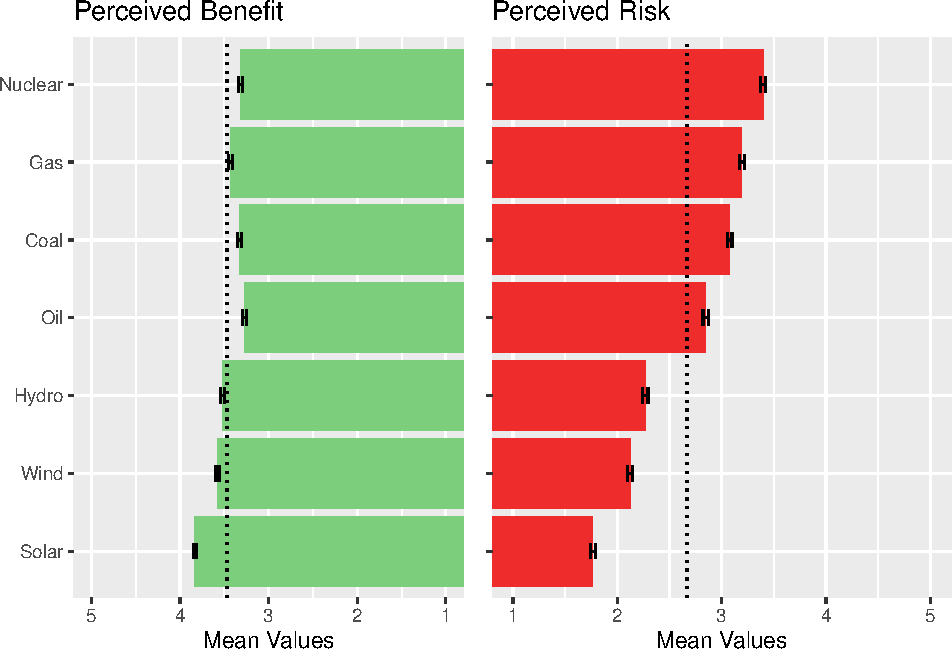
\includegraphics{Paper1_files/figure-latex/unnamed-chunk-6-1.pdf}

\newpage

\hypertarget{h2-gender-and-caste-will-have-significant-impact-like-gender-and-race-in-the-us-studies-of-risk.}{%
\section{H2: Gender and Caste will have significant impact like Gender
and Race in the US studies of
risk.}\label{h2-gender-and-caste-will-have-significant-impact-like-gender-and-race-in-the-us-studies-of-risk.}}

\begin{verbatim}
## 
## Call:
## lm(formula = Risky_Nuclear ~ Uppercaste + Male + Hindu + Urban + 
##     age, data = alldemos)
## 
## Residuals:
##     Min      1Q  Median      3Q     Max 
## -2.6471 -1.1853  0.2939  0.7328  1.8294 
## 
## Coefficients:
##             Estimate Std. Error t value Pr(>|t|)    
## (Intercept)  3.35999    0.10432  32.209   <2e-16 ***
## Uppercaste   0.14139    0.06439   2.196   0.0282 *  
## Male         0.13101    0.06409   2.044   0.0411 *  
## Hindu       -0.12223    0.07561  -1.617   0.1062    
## UrbanUrban  -0.08190    0.06283  -1.304   0.1926    
## age          0.01475    0.02711   0.544   0.5866    
## ---
## Signif. codes:  0 '***' 0.001 '**' 0.01 '*' 0.05 '.' 0.1 ' ' 1
## 
## Residual standard error: 1.184 on 1548 degrees of freedom
##   (607 observations deleted due to missingness)
## Multiple R-squared:  0.01055,    Adjusted R-squared:  0.007356 
## F-statistic: 3.302 on 5 and 1548 DF,  p-value: 0.005702
\end{verbatim}

\begin{verbatim}
## 
## Call:
## lm(formula = Risky_Nuclear ~ Uppercaste + Male + Hindu + Urban + 
##     age + State, data = alldemos)
## 
## Residuals:
##     Min      1Q  Median      3Q     Max 
## -3.2394 -0.8825 -0.1205  0.7704  2.2064 
## 
## Coefficients:
##                    Estimate Std. Error t value Pr(>|t|)    
## (Intercept)         3.20856    0.09587  33.466  < 2e-16 ***
## Uppercaste         -0.11678    0.05915  -1.974  0.04854 *  
## Male                0.02336    0.05937   0.394  0.69399    
## Hindu              -0.03235    0.06875  -0.471  0.63798    
## UrbanUrban          0.08122    0.06376   1.274  0.20293    
## age                -0.02786    0.02519  -1.106  0.26881    
## StateRajasthan      0.24549    0.09271   2.648  0.00818 ** 
## StateTamil Nadu    -0.23347    0.08677  -2.691  0.00721 ** 
## StateUttar Pradesh -0.15431    0.11865  -1.301  0.19361    
## StateWest Bengal    1.31933    0.08104  16.280  < 2e-16 ***
## ---
## Signif. codes:  0 '***' 0.001 '**' 0.01 '*' 0.05 '.' 0.1 ' ' 1
## 
## Residual standard error: 1.056 on 1544 degrees of freedom
##   (607 observations deleted due to missingness)
## Multiple R-squared:  0.2147, Adjusted R-squared:  0.2102 
## F-statistic: 46.91 on 9 and 1544 DF,  p-value: < 2.2e-16
\end{verbatim}

\hypertarget{two-linear-regression-models}{%
\subsection{two linear regression
models}\label{two-linear-regression-models}}

\begingroup\setlength{\tabcolsep}{1pt}\renewcommand{\arraystretch}{0.7}

\% Table created by stargazer v.5.2.3 by Marek Hlavac, Social Policy
Institute. E-mail: marek.hlavac at gmail.com \% Date and time: Sat, Jan
13, 2024 - 17:42:11

\begin{table}[!htbp] \centering 
  \caption{Results from 2 linear regression models} 
  \label{} 
\begin{tabular}{@{\extracolsep{5pt}}lcc} 
\\[-1.8ex]\hline 
\hline \\[-1.8ex] 
 & \multicolumn{2}{c}{\textit{Dependent variable:}} \\ 
\cline{2-3} 
\\[-1.8ex] & \multicolumn{2}{c}{Risky\_Nuclear} \\ 
\\[-1.8ex] & (1) & (2)\\ 
\hline \\[-1.8ex] 
 Uppercaste & 0.141$^{**}$ & $-$0.117$^{**}$ \\ 
  & (0.064) & (0.059) \\ 
  & & \\ 
 Male & 0.131$^{**}$ & 0.023 \\ 
  & (0.064) & (0.059) \\ 
  & & \\ 
 Hindu & $-$0.122 & $-$0.032 \\ 
  & (0.076) & (0.069) \\ 
  & & \\ 
 UrbanUrban & $-$0.082 & 0.081 \\ 
  & (0.063) & (0.064) \\ 
  & & \\ 
 age & 0.015 & $-$0.028 \\ 
  & (0.027) & (0.025) \\ 
  & & \\ 
 StateRajasthan &  & 0.245$^{***}$ \\ 
  &  & (0.093) \\ 
  & & \\ 
 StateTamil Nadu &  & $-$0.233$^{***}$ \\ 
  &  & (0.087) \\ 
  & & \\ 
 StateUttar Pradesh &  & $-$0.154 \\ 
  &  & (0.119) \\ 
  & & \\ 
 StateWest Bengal &  & 1.319$^{***}$ \\ 
  &  & (0.081) \\ 
  & & \\ 
 Constant & 3.360$^{***}$ & 3.209$^{***}$ \\ 
  & (0.104) & (0.096) \\ 
  & & \\ 
\hline \\[-1.8ex] 
Observations & 1,554 & 1,554 \\ 
R$^{2}$ & 0.011 & 0.215 \\ 
Adjusted R$^{2}$ & 0.007 & 0.210 \\ 
Residual Std. Error & 1.184 (df = 1548) & 1.056 (df = 1544) \\ 
F Statistic & 3.302$^{***}$ (df = 5; 1548) & 46.913$^{***}$ (df = 9; 1544) \\ 
\hline 
\hline \\[-1.8ex] 
\textit{Note:}  & \multicolumn{2}{r}{$^{*}$p$<$0.1; $^{**}$p$<$0.05; $^{***}$p$<$0.01} \\ 
\end{tabular} 
\end{table} 
\endgroup

\newpage

\hypertarget{h3-regional-differences-will-have-a-strong-impact}{%
\section{H3: Regional differences will have a strong
impact}\label{h3-regional-differences-will-have-a-strong-impact}}

\hypertarget{linear-regression-where-mean-value-is-the-intercept}{%
\subsection{Linear regression where Mean value is the
intercept}\label{linear-regression-where-mean-value-is-the-intercept}}

Same model with mean value as intercept.

\newpage

\hypertarget{regional-differences-graph}{%
\subsection{Regional Differences
Graph}\label{regional-differences-graph}}

Following is a graph of z scores calculated from mean perceived risk
from nuclear energy by state.

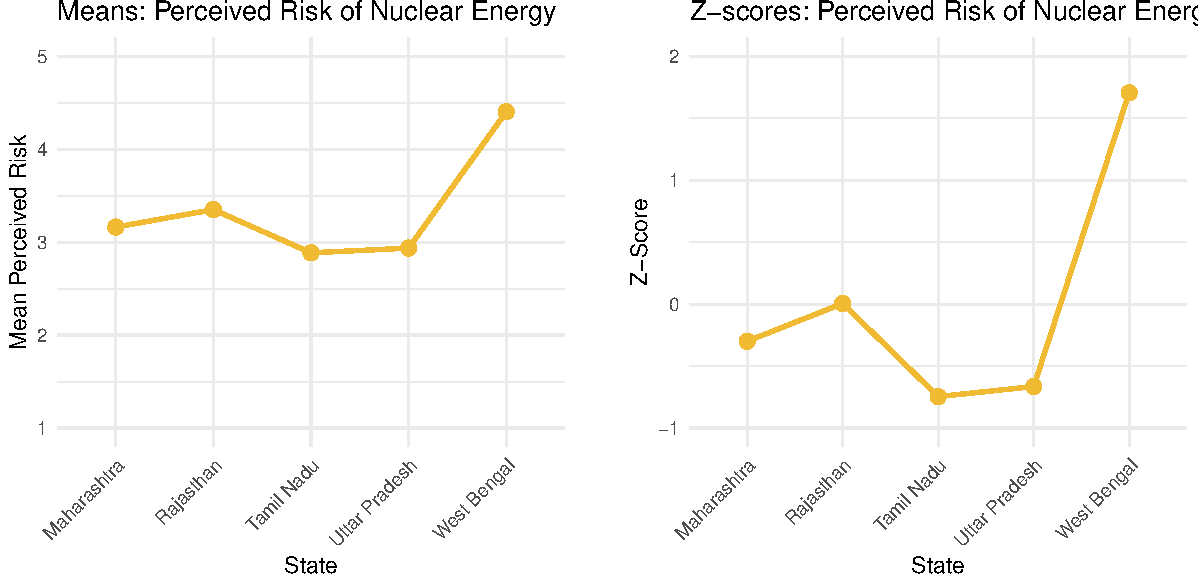
\includegraphics{Paper1_files/figure-latex/unnamed-chunk-12-1.pdf}

\newpage

\hypertarget{confirmatory-factor-analysiscfa-kahan-scale}{%
\section{Confirmatory Factor Analysis(CFA): Kahan
Scale}\label{confirmatory-factor-analysiscfa-kahan-scale}}

\textbf{Cronbach's Alpha on Kahan et al(2007) Scale: A Note}

The Individualism items (indicated by K\_I) were bringing down the
Cronbach's alpha values in the Kahan scale. The Alpha for Individualism-
Communitarian scale was 0.49. After removing the Individualism items
(K\_I) the alpha for this factor was 0.71. The reasons for this could be
that the individualism items are not well adapted to the Indian
population.

\begin{table}[!h]

\caption{\label{tab:unnamed-chunk-14}Fit Measures from the CFA}
\centering
\begin{tabular}[t]{lr}
\toprule
Measure & Value\\
\midrule
\cellcolor{gray!6}{Comparative Fit Index (CFI)} & \cellcolor{gray!6}{0.954}\\
Tucker-Lewis Index (TLI) & 0.925\\
\cellcolor{gray!6}{Root Mean Square Error of Approximation(RMSEA)} & \cellcolor{gray!6}{0.074}\\
RMSEA 90 Percent confidence interval - lower & 0.100\\
\cellcolor{gray!6}{RMSEA 90 Percent confidence interval - upper} & \cellcolor{gray!6}{0.050}\\
\bottomrule
\end{tabular}
\end{table}

\newpage

\begin{landscape}\begin{table}[!h]

\caption{\label{tab:unnamed-chunk-15}Confirmatory Factor Analysis(CFA) on Kahan et al(2007) scale adapted to India}
\centering
\resizebox{\linewidth}{!}{
\begin{tabular}[t]{l>{\raggedright\arraybackslash}p{4cm}rrrrrrrr}
\toprule
Scale & Items & Loadings & Standard Error & zvalue & pvalue & ci.lower & ci.upper & std.lv & std.all\\
\midrule
\cellcolor{gray!6}{Communitarian} & \cellcolor{gray!6}{Sometimes the government needs to make laws that keep people from hurting themselves.} & \cellcolor{gray!6}{0.704} & \cellcolor{gray!6}{0.064} & \cellcolor{gray!6}{11.037} & \cellcolor{gray!6}{0} & \cellcolor{gray!6}{0.5786531} & \cellcolor{gray!6}{0.8285358} & \cellcolor{gray!6}{0.7035944} & \cellcolor{gray!6}{0.6207523}\\
Communitarian & The government should put limits on the choices individuals can make so they don’t get in the way of what’s good for society. & 0.765 & 0.066 & 11.655 & 0 & 0.6366205 & 0.8940208 & 0.7653206 & 0.6579374\\
\cellcolor{gray!6}{Communitarian} & \cellcolor{gray!6}{The government should do more to advance society’s goals, even if that means limiting the freedom and choices of individuals.} & \cellcolor{gray!6}{0.546} & \cellcolor{gray!6}{0.065} & \cellcolor{gray!6}{8.385} & \cellcolor{gray!6}{0} & \cellcolor{gray!6}{0.4184991} & \cellcolor{gray!6}{0.6738458} & \cellcolor{gray!6}{0.5461725} & \cellcolor{gray!6}{0.4767128}\\
Hierarchy-Egalitarianism & We have gone too far in pushing equal rights in this country. & 0.686 & 0.062 & 11.139 & 0 & 0.5656331 & 0.8071956 & 0.6864143 & 0.5687108\\
\cellcolor{gray!6}{Hierarchy-Egalitarianism} & \cellcolor{gray!6}{We need to dramatically reduce inequalities between the rich and the poor.} & \cellcolor{gray!6}{-0.803} & \cellcolor{gray!6}{0.052} & \cellcolor{gray!6}{-15.402} & \cellcolor{gray!6}{0} & \cellcolor{gray!6}{-0.9054554} & \cellcolor{gray!6}{-0.7010198} & \cellcolor{gray!6}{-0.8032376} & \cellcolor{gray!6}{-0.7469721}\\
\addlinespace
Hierarchy-Egalitarianism & Our society would be better off if the distribution of wealth was more equal. & -0.640 & 0.061 & -10.478 & 0 & -0.7600516 & -0.5205128 & -0.6402822 & -0.5396459\\
\cellcolor{gray!6}{Hierarchy-Egalitarianism} & \cellcolor{gray!6}{We need to dramatically reduce inequalities between men and women.} & \cellcolor{gray!6}{-0.857} & \cellcolor{gray!6}{0.055} & \cellcolor{gray!6}{-15.539} & \cellcolor{gray!6}{0} & \cellcolor{gray!6}{-0.9650777} & \cellcolor{gray!6}{-0.7488861} & \cellcolor{gray!6}{-0.8569819} & \cellcolor{gray!6}{-0.7525525}\\
\bottomrule
\end{tabular}}
\end{table}
\end{landscape}

\newpage

\hypertarget{factor-analysis-new-eco-political-scale}{%
\section{Factor Analysis: New Eco-political
Scale}\label{factor-analysis-new-eco-political-scale}}

\begin{verbatim}
## Factor Analysis using method =  minres
## Call: fa(r = ecopolall, nfactors = 2, rotate = "varimax")
## Standardized loadings (pattern matrix) based upon correlation matrix
##                 item   MR1   MR2     h2   u2 com
## HEALTHNUCLEAR     17  0.66  0.06 0.4352 0.56 1.0
## BEAUTYNUCLEAR     19  0.64  0.06 0.4104 0.59 1.0
## DISPLACENUCLEAR   15  0.59  0.18 0.3795 0.62 1.2
## POLLUTENUCLEAR    16  0.56  0.00 0.3188 0.68 1.0
## MECHANISATION      2  0.55  0.20 0.3454 0.65 1.3
## INDUSTRYSMALL      6  0.53  0.02 0.2840 0.72 1.0
## OWNERREG          14  0.53  0.10 0.2905 0.71 1.1
## ENVOVERDEV         9  0.39  0.02 0.1529 0.85 1.0
## ECONOMYGLOBAL      7 -0.34 -0.32 0.2179 0.78 2.0
## OWNERPUB          13  0.33  0.11 0.1228 0.88 1.2
## DECISIONDECEN      3  0.29  0.00 0.0840 0.92 1.0
## WEALTHLIM          1  0.27  0.27 0.1437 0.86 2.0
## OWNERPVT          11 -0.13 -0.11 0.0311 0.97 1.9
## ECONOMYLOCAL       8  0.12  0.02 0.0147 0.99 1.0
## DEVNUCLEAR        22  0.19  0.66 0.4730 0.53 1.2
## PRIDENUCLEAR      20 -0.21  0.62 0.4341 0.57 1.2
## NPRIDENUCLEAR     21 -0.19  0.61 0.4023 0.60 1.2
## PROSPERNUCLEAR    23  0.13  0.59 0.3602 0.64 1.1
## JOBSNUCLEAR       18  0.21  0.43 0.2264 0.77 1.5
## RELYNUCLEAR       24  0.06  0.39 0.1557 0.84 1.0
## INDUSTRYLARGE      5 -0.23 -0.34 0.1730 0.83 1.8
## OWNERNOREG        12 -0.11 -0.24 0.0688 0.93 1.4
## DECISIONCEN        4 -0.18 -0.22 0.0834 0.92 1.9
## DEVOVERENV        10  0.01 -0.07 0.0043 1.00 1.0
## 
##                        MR1  MR2
## SS loadings           3.22 2.39
## Proportion Var        0.13 0.10
## Cumulative Var        0.13 0.23
## Proportion Explained  0.57 0.43
## Cumulative Proportion 0.57 1.00
## 
## Mean item complexity =  1.3
## Test of the hypothesis that 2 factors are sufficient.
## 
## df null model =  276  with the objective function =  5.93 with Chi Square =  2343.45
## df of  the model are 229  and the objective function was  2.35 
## 
## The root mean square of the residuals (RMSR) is  0.08 
## The df corrected root mean square of the residuals is  0.08 
## 
## The harmonic n.obs is  405 with the empirical chi square  1307.09  with prob <  2.6e-150 
## The total n.obs was  405  with Likelihood Chi Square =  924.07  with prob <  3.4e-84 
## 
## Tucker Lewis Index of factoring reliability =  0.593
## RMSEA index =  0.087  and the 90 % confidence intervals are  0.081 0.093
## BIC =  -450.82
## Fit based upon off diagonal values = 0.83
## Measures of factor score adequacy             
##                                                    MR1  MR2
## Correlation of (regression) scores with factors   0.91 0.88
## Multiple R square of scores with factors          0.82 0.78
## Minimum correlation of possible factor scores     0.64 0.56
\end{verbatim}

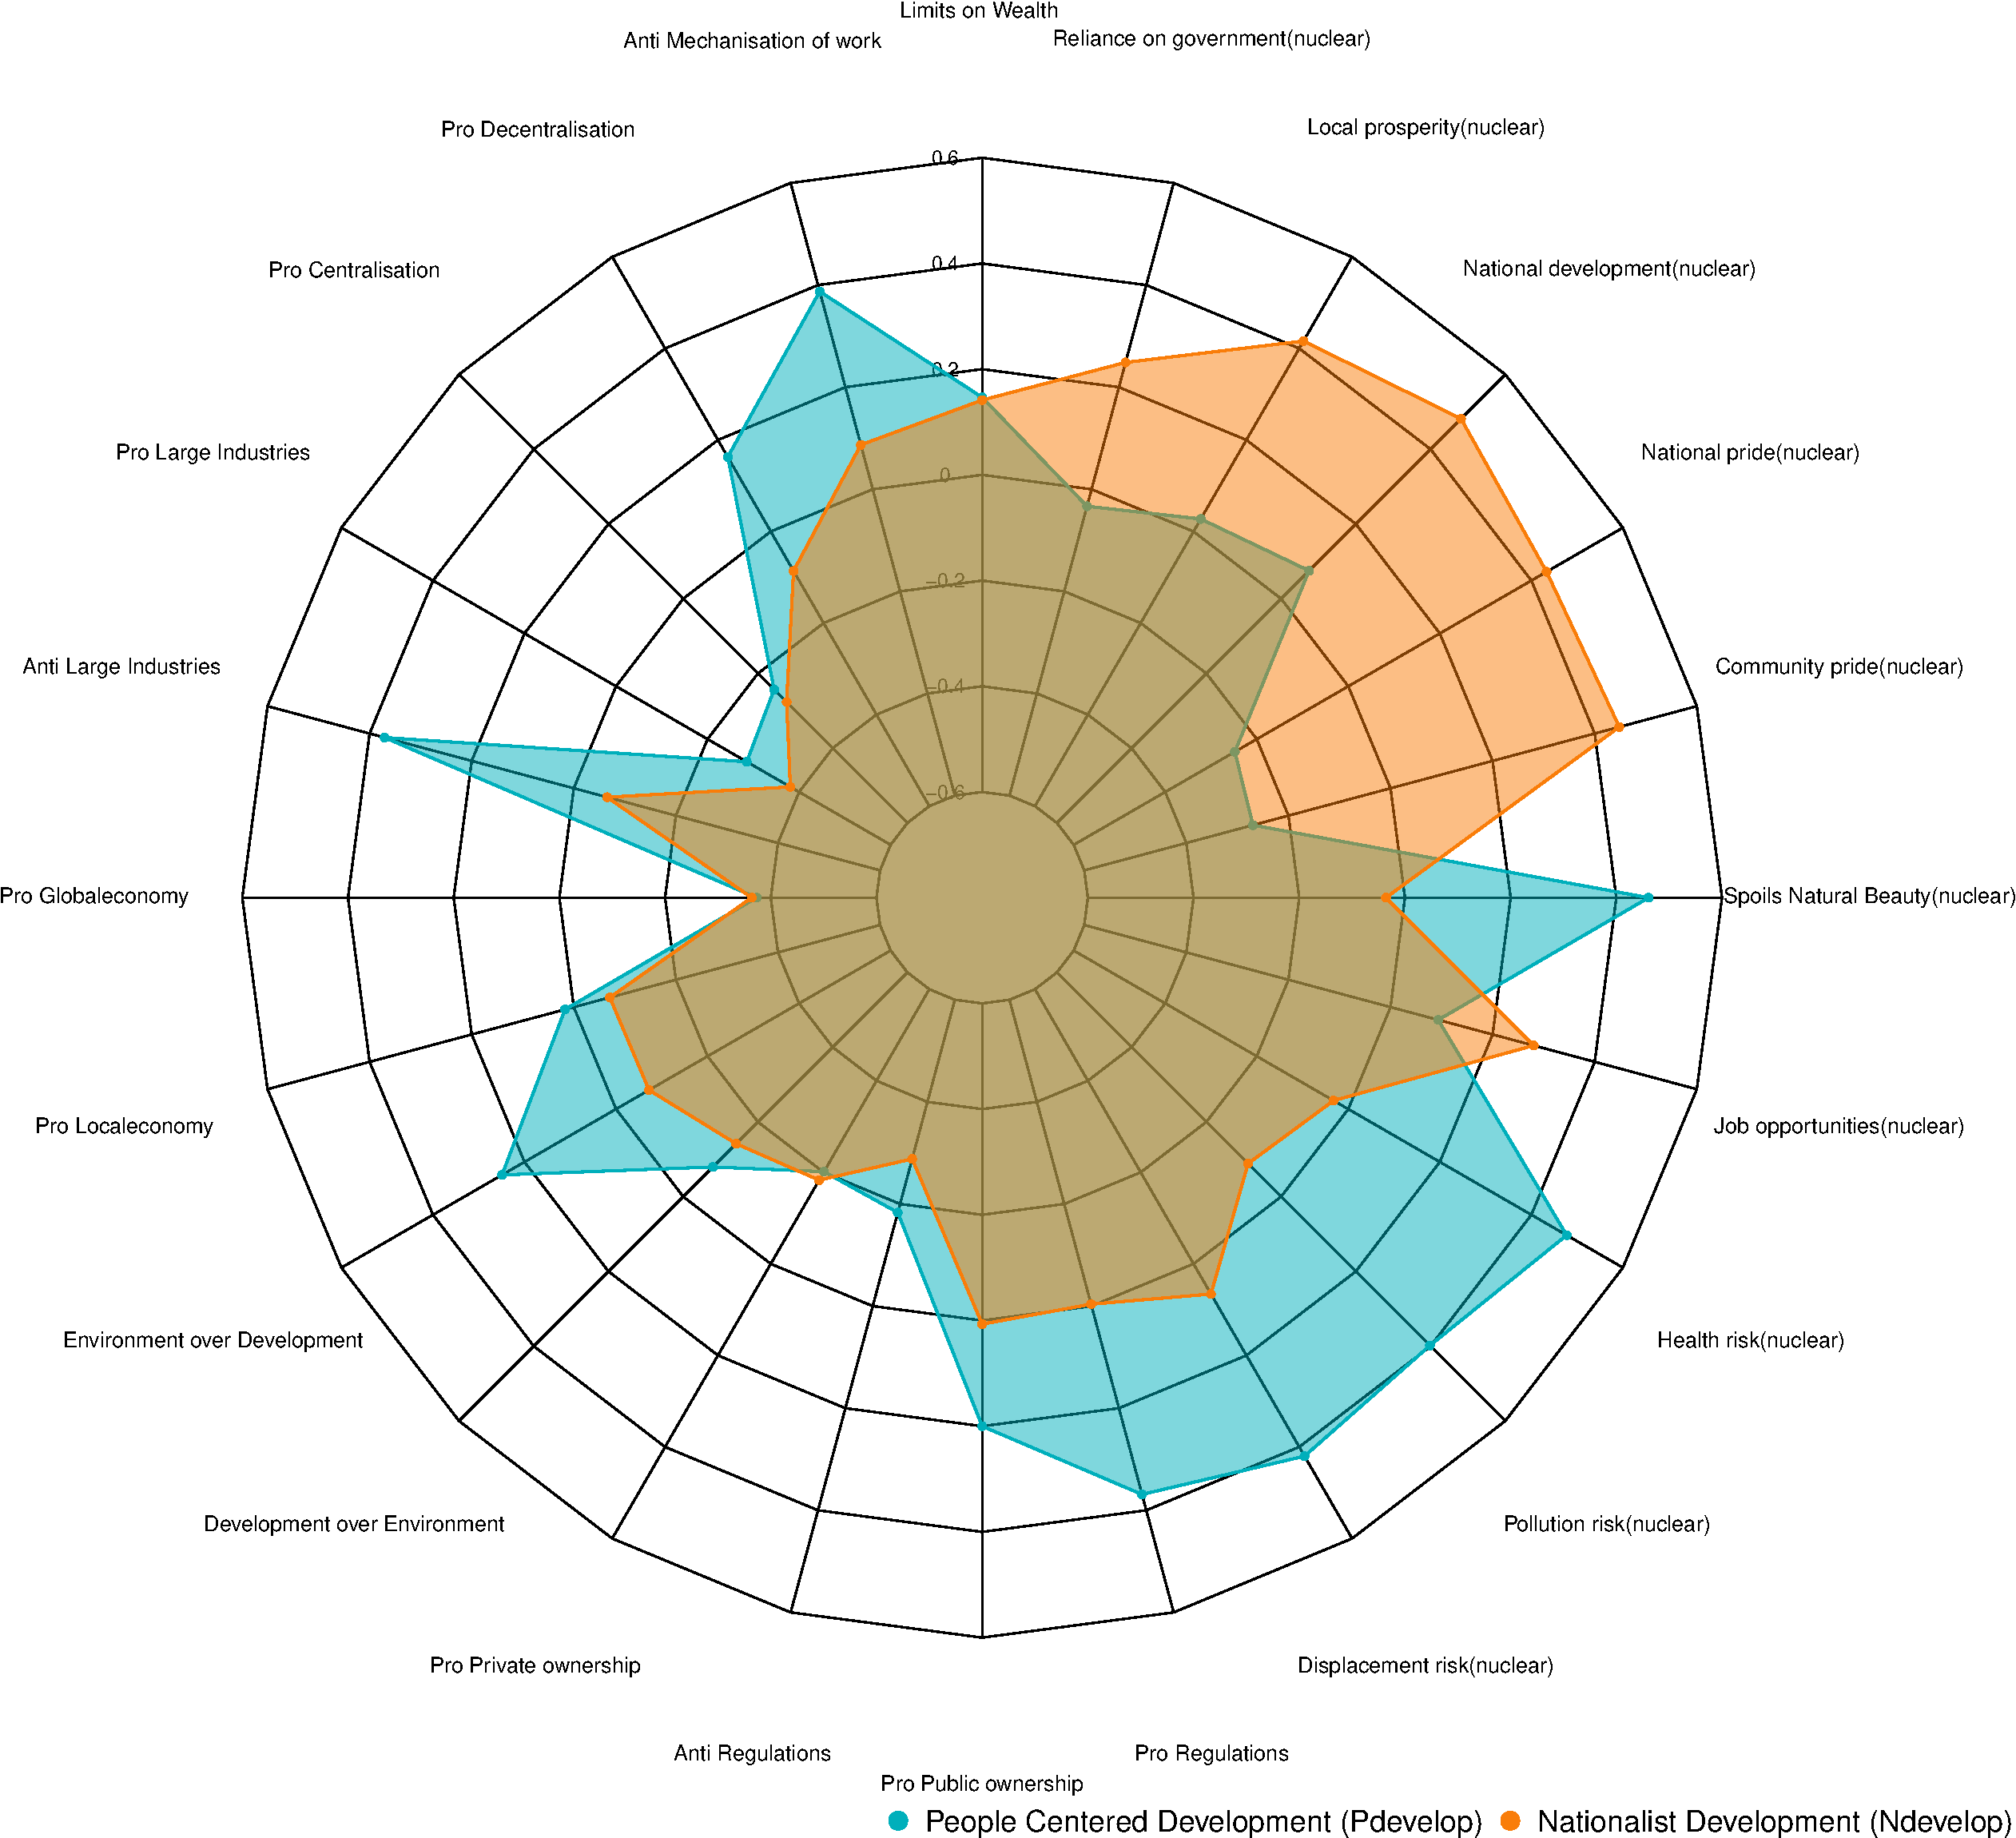
\includegraphics[width=1\linewidth,height=1\textheight]{Paper1_files/figure-latex/unnamed-chunk-18-1}

\newpage

\global\setlength{\Oldarrayrulewidth}{\arrayrulewidth}

\global\setlength{\Oldtabcolsep}{\tabcolsep}

\setlength{\tabcolsep}{0pt}

\renewcommand*{\arraystretch}{1.5}



\providecommand{\ascline}[3]{\noalign{\global\arrayrulewidth #1}\arrayrulecolor[HTML]{#2}\cline{#3}}

\begin{longtable}[c]{cccccc}

\caption{Eco-Pol\ Values\ Factor\ Analysis\ Table}\\

\ascline{1.5pt}{666666}{1-6}

\multicolumn{1}{>{}l}{\textcolor[HTML]{000000}{\fontsize{10}{10}\selectfont{Items}}} & \multicolumn{1}{>{}r}{\textcolor[HTML]{000000}{\fontsize{10}{10}\selectfont{Pdevelop}}} & \multicolumn{1}{>{}r}{\textcolor[HTML]{000000}{\fontsize{10}{10}\selectfont{Ndevelop}}} & \multicolumn{1}{>{}r}{\textcolor[HTML]{000000}{\fontsize{10}{10}\selectfont{Communality}}} & \multicolumn{1}{>{}r}{\textcolor[HTML]{000000}{\fontsize{10}{10}\selectfont{Uniqueness}}} & \multicolumn{1}{>{}r}{\textcolor[HTML]{000000}{\fontsize{10}{10}\selectfont{Complexity}}} \\

\ascline{1.5pt}{666666}{1-6}\endfirsthead \caption[]{Eco-Pol\ Values\ Factor\ Analysis\ Table}\\

\ascline{1.5pt}{666666}{1-6}

\multicolumn{1}{>{}l}{\textcolor[HTML]{000000}{\fontsize{10}{10}\selectfont{Items}}} & \multicolumn{1}{>{}r}{\textcolor[HTML]{000000}{\fontsize{10}{10}\selectfont{Pdevelop}}} & \multicolumn{1}{>{}r}{\textcolor[HTML]{000000}{\fontsize{10}{10}\selectfont{Ndevelop}}} & \multicolumn{1}{>{}r}{\textcolor[HTML]{000000}{\fontsize{10}{10}\selectfont{Communality}}} & \multicolumn{1}{>{}r}{\textcolor[HTML]{000000}{\fontsize{10}{10}\selectfont{Uniqueness}}} & \multicolumn{1}{>{}r}{\textcolor[HTML]{000000}{\fontsize{10}{10}\selectfont{Complexity}}} \\

\ascline{1.5pt}{666666}{1-6}\endhead



\multicolumn{1}{>{}l}{\textcolor[HTML]{000000}{\fontsize{10}{10}\selectfont{Health\ risk(nuclear)}}} & \multicolumn{1}{>{}r}{\textcolor[HTML]{000000}{\fontsize{10}{10}\selectfont{0.657}}} & \multicolumn{1}{>{}r}{\textcolor[HTML]{000000}{\fontsize{10}{10}\selectfont{0.062}}} & \multicolumn{1}{>{}r}{\textcolor[HTML]{000000}{\fontsize{10}{10}\selectfont{0.435}}} & \multicolumn{1}{>{}r}{\textcolor[HTML]{000000}{\fontsize{10}{10}\selectfont{0.565}}} & \multicolumn{1}{>{}r}{\textcolor[HTML]{000000}{\fontsize{10}{10}\selectfont{1.018}}} \\





\multicolumn{1}{>{}l}{\textcolor[HTML]{000000}{\fontsize{10}{10}\selectfont{Spoils\ Natural\ Beauty(nuclear)}}} & \multicolumn{1}{>{}r}{\textcolor[HTML]{000000}{\fontsize{10}{10}\selectfont{0.638}}} & \multicolumn{1}{>{}r}{\textcolor[HTML]{000000}{\fontsize{10}{10}\selectfont{0.058}}} & \multicolumn{1}{>{}r}{\textcolor[HTML]{000000}{\fontsize{10}{10}\selectfont{0.410}}} & \multicolumn{1}{>{}r}{\textcolor[HTML]{000000}{\fontsize{10}{10}\selectfont{0.590}}} & \multicolumn{1}{>{}r}{\textcolor[HTML]{000000}{\fontsize{10}{10}\selectfont{1.017}}} \\





\multicolumn{1}{>{}l}{\textcolor[HTML]{000000}{\fontsize{10}{10}\selectfont{Displacement\ risk(nuclear)}}} & \multicolumn{1}{>{}r}{\textcolor[HTML]{000000}{\fontsize{10}{10}\selectfont{0.590}}} & \multicolumn{1}{>{}r}{\textcolor[HTML]{000000}{\fontsize{10}{10}\selectfont{0.177}}} & \multicolumn{1}{>{}r}{\textcolor[HTML]{000000}{\fontsize{10}{10}\selectfont{0.380}}} & \multicolumn{1}{>{}r}{\textcolor[HTML]{000000}{\fontsize{10}{10}\selectfont{0.620}}} & \multicolumn{1}{>{}r}{\textcolor[HTML]{000000}{\fontsize{10}{10}\selectfont{1.178}}} \\





\multicolumn{1}{>{}l}{\textcolor[HTML]{000000}{\fontsize{10}{10}\selectfont{Pollution\ risk(nuclear)}}} & \multicolumn{1}{>{}r}{\textcolor[HTML]{000000}{\fontsize{10}{10}\selectfont{0.565}}} & \multicolumn{1}{>{}r}{\textcolor[HTML]{000000}{\fontsize{10}{10}\selectfont{-0.003}}} & \multicolumn{1}{>{}r}{\textcolor[HTML]{000000}{\fontsize{10}{10}\selectfont{0.319}}} & \multicolumn{1}{>{}r}{\textcolor[HTML]{000000}{\fontsize{10}{10}\selectfont{0.681}}} & \multicolumn{1}{>{}r}{\textcolor[HTML]{000000}{\fontsize{10}{10}\selectfont{1.000}}} \\





\multicolumn{1}{>{}l}{\textcolor[HTML]{000000}{\fontsize{10}{10}\selectfont{Anti\ Mechanisation\ of\ work}}} & \multicolumn{1}{>{}r}{\textcolor[HTML]{000000}{\fontsize{10}{10}\selectfont{0.552}}} & \multicolumn{1}{>{}r}{\textcolor[HTML]{000000}{\fontsize{10}{10}\selectfont{0.201}}} & \multicolumn{1}{>{}r}{\textcolor[HTML]{000000}{\fontsize{10}{10}\selectfont{0.345}}} & \multicolumn{1}{>{}r}{\textcolor[HTML]{000000}{\fontsize{10}{10}\selectfont{0.655}}} & \multicolumn{1}{>{}r}{\textcolor[HTML]{000000}{\fontsize{10}{10}\selectfont{1.262}}} \\





\multicolumn{1}{>{}l}{\textcolor[HTML]{000000}{\fontsize{10}{10}\selectfont{Anti\ Large\ Industries}}} & \multicolumn{1}{>{}r}{\textcolor[HTML]{000000}{\fontsize{10}{10}\selectfont{0.532}}} & \multicolumn{1}{>{}r}{\textcolor[HTML]{000000}{\fontsize{10}{10}\selectfont{0.024}}} & \multicolumn{1}{>{}r}{\textcolor[HTML]{000000}{\fontsize{10}{10}\selectfont{0.284}}} & \multicolumn{1}{>{}r}{\textcolor[HTML]{000000}{\fontsize{10}{10}\selectfont{0.716}}} & \multicolumn{1}{>{}r}{\textcolor[HTML]{000000}{\fontsize{10}{10}\selectfont{1.004}}} \\





\multicolumn{1}{>{}l}{\textcolor[HTML]{000000}{\fontsize{10}{10}\selectfont{Pro\ Regulations}}} & \multicolumn{1}{>{}r}{\textcolor[HTML]{000000}{\fontsize{10}{10}\selectfont{0.530}}} & \multicolumn{1}{>{}r}{\textcolor[HTML]{000000}{\fontsize{10}{10}\selectfont{0.096}}} & \multicolumn{1}{>{}r}{\textcolor[HTML]{000000}{\fontsize{10}{10}\selectfont{0.290}}} & \multicolumn{1}{>{}r}{\textcolor[HTML]{000000}{\fontsize{10}{10}\selectfont{0.710}}} & \multicolumn{1}{>{}r}{\textcolor[HTML]{000000}{\fontsize{10}{10}\selectfont{1.065}}} \\





\multicolumn{1}{>{}l}{\textcolor[HTML]{000000}{\fontsize{10}{10}\selectfont{Environment\ over\ Development}}} & \multicolumn{1}{>{}r}{\textcolor[HTML]{000000}{\fontsize{10}{10}\selectfont{0.391}}} & \multicolumn{1}{>{}r}{\textcolor[HTML]{000000}{\fontsize{10}{10}\selectfont{0.016}}} & \multicolumn{1}{>{}r}{\textcolor[HTML]{000000}{\fontsize{10}{10}\selectfont{0.153}}} & \multicolumn{1}{>{}r}{\textcolor[HTML]{000000}{\fontsize{10}{10}\selectfont{0.847}}} & \multicolumn{1}{>{}r}{\textcolor[HTML]{000000}{\fontsize{10}{10}\selectfont{1.003}}} \\





\multicolumn{1}{>{}l}{\textcolor[HTML]{000000}{\fontsize{10}{10}\selectfont{Pro\ Globaleconomy}}} & \multicolumn{1}{>{}r}{\textcolor[HTML]{000000}{\fontsize{10}{10}\selectfont{-0.335}}} & \multicolumn{1}{>{}r}{\textcolor[HTML]{000000}{\fontsize{10}{10}\selectfont{-0.325}}} & \multicolumn{1}{>{}r}{\textcolor[HTML]{000000}{\fontsize{10}{10}\selectfont{0.218}}} & \multicolumn{1}{>{}r}{\textcolor[HTML]{000000}{\fontsize{10}{10}\selectfont{0.782}}} & \multicolumn{1}{>{}r}{\textcolor[HTML]{000000}{\fontsize{10}{10}\selectfont{1.998}}} \\





\multicolumn{1}{>{}l}{\textcolor[HTML]{000000}{\fontsize{10}{10}\selectfont{Pro\ Public\ ownership}}} & \multicolumn{1}{>{}r}{\textcolor[HTML]{000000}{\fontsize{10}{10}\selectfont{0.333}}} & \multicolumn{1}{>{}r}{\textcolor[HTML]{000000}{\fontsize{10}{10}\selectfont{0.108}}} & \multicolumn{1}{>{}r}{\textcolor[HTML]{000000}{\fontsize{10}{10}\selectfont{0.123}}} & \multicolumn{1}{>{}r}{\textcolor[HTML]{000000}{\fontsize{10}{10}\selectfont{0.877}}} & \multicolumn{1}{>{}r}{\textcolor[HTML]{000000}{\fontsize{10}{10}\selectfont{1.208}}} \\





\multicolumn{1}{>{}l}{\textcolor[HTML]{000000}{\fontsize{10}{10}\selectfont{Pro\ Decentralisation}}} & \multicolumn{1}{>{}r}{\textcolor[HTML]{000000}{\fontsize{10}{10}\selectfont{0.290}}} & \multicolumn{1}{>{}r}{\textcolor[HTML]{000000}{\fontsize{10}{10}\selectfont{-0.001}}} & \multicolumn{1}{>{}r}{\textcolor[HTML]{000000}{\fontsize{10}{10}\selectfont{0.084}}} & \multicolumn{1}{>{}r}{\textcolor[HTML]{000000}{\fontsize{10}{10}\selectfont{0.916}}} & \multicolumn{1}{>{}r}{\textcolor[HTML]{000000}{\fontsize{10}{10}\selectfont{1.000}}} \\





\multicolumn{1}{>{}l}{\textcolor[HTML]{000000}{\fontsize{10}{10}\selectfont{Limits\ on\ Wealth}}} & \multicolumn{1}{>{}r}{\textcolor[HTML]{000000}{\fontsize{10}{10}\selectfont{0.271}}} & \multicolumn{1}{>{}r}{\textcolor[HTML]{000000}{\fontsize{10}{10}\selectfont{0.265}}} & \multicolumn{1}{>{}r}{\textcolor[HTML]{000000}{\fontsize{10}{10}\selectfont{0.144}}} & \multicolumn{1}{>{}r}{\textcolor[HTML]{000000}{\fontsize{10}{10}\selectfont{0.856}}} & \multicolumn{1}{>{}r}{\textcolor[HTML]{000000}{\fontsize{10}{10}\selectfont{1.999}}} \\





\multicolumn{1}{>{}l}{\textcolor[HTML]{000000}{\fontsize{10}{10}\selectfont{Pro\ Private\ ownership}}} & \multicolumn{1}{>{}r}{\textcolor[HTML]{000000}{\fontsize{10}{10}\selectfont{-0.135}}} & \multicolumn{1}{>{}r}{\textcolor[HTML]{000000}{\fontsize{10}{10}\selectfont{-0.113}}} & \multicolumn{1}{>{}r}{\textcolor[HTML]{000000}{\fontsize{10}{10}\selectfont{0.031}}} & \multicolumn{1}{>{}r}{\textcolor[HTML]{000000}{\fontsize{10}{10}\selectfont{0.969}}} & \multicolumn{1}{>{}r}{\textcolor[HTML]{000000}{\fontsize{10}{10}\selectfont{1.943}}} \\





\multicolumn{1}{>{}l}{\textcolor[HTML]{000000}{\fontsize{10}{10}\selectfont{Pro\ Localeconomy}}} & \multicolumn{1}{>{}r}{\textcolor[HTML]{000000}{\fontsize{10}{10}\selectfont{0.120}}} & \multicolumn{1}{>{}r}{\textcolor[HTML]{000000}{\fontsize{10}{10}\selectfont{0.018}}} & \multicolumn{1}{>{}r}{\textcolor[HTML]{000000}{\fontsize{10}{10}\selectfont{0.015}}} & \multicolumn{1}{>{}r}{\textcolor[HTML]{000000}{\fontsize{10}{10}\selectfont{0.985}}} & \multicolumn{1}{>{}r}{\textcolor[HTML]{000000}{\fontsize{10}{10}\selectfont{1.043}}} \\





\multicolumn{1}{>{}l}{\textcolor[HTML]{000000}{\fontsize{10}{10}\selectfont{National\ development(nuclear)}}} & \multicolumn{1}{>{}r}{\textcolor[HTML]{000000}{\fontsize{10}{10}\selectfont{0.187}}} & \multicolumn{1}{>{}r}{\textcolor[HTML]{000000}{\fontsize{10}{10}\selectfont{0.662}}} & \multicolumn{1}{>{}r}{\textcolor[HTML]{000000}{\fontsize{10}{10}\selectfont{0.473}}} & \multicolumn{1}{>{}r}{\textcolor[HTML]{000000}{\fontsize{10}{10}\selectfont{0.527}}} & \multicolumn{1}{>{}r}{\textcolor[HTML]{000000}{\fontsize{10}{10}\selectfont{1.159}}} \\





\multicolumn{1}{>{}l}{\textcolor[HTML]{000000}{\fontsize{10}{10}\selectfont{Community\ pride(nuclear)}}} & \multicolumn{1}{>{}r}{\textcolor[HTML]{000000}{\fontsize{10}{10}\selectfont{-0.215}}} & \multicolumn{1}{>{}r}{\textcolor[HTML]{000000}{\fontsize{10}{10}\selectfont{0.623}}} & \multicolumn{1}{>{}r}{\textcolor[HTML]{000000}{\fontsize{10}{10}\selectfont{0.434}}} & \multicolumn{1}{>{}r}{\textcolor[HTML]{000000}{\fontsize{10}{10}\selectfont{0.566}}} & \multicolumn{1}{>{}r}{\textcolor[HTML]{000000}{\fontsize{10}{10}\selectfont{1.234}}} \\





\multicolumn{1}{>{}l}{\textcolor[HTML]{000000}{\fontsize{10}{10}\selectfont{National\ pride(nuclear)}}} & \multicolumn{1}{>{}r}{\textcolor[HTML]{000000}{\fontsize{10}{10}\selectfont{-0.189}}} & \multicolumn{1}{>{}r}{\textcolor[HTML]{000000}{\fontsize{10}{10}\selectfont{0.605}}} & \multicolumn{1}{>{}r}{\textcolor[HTML]{000000}{\fontsize{10}{10}\selectfont{0.402}}} & \multicolumn{1}{>{}r}{\textcolor[HTML]{000000}{\fontsize{10}{10}\selectfont{0.598}}} & \multicolumn{1}{>{}r}{\textcolor[HTML]{000000}{\fontsize{10}{10}\selectfont{1.193}}} \\





\multicolumn{1}{>{}l}{\textcolor[HTML]{000000}{\fontsize{10}{10}\selectfont{Local\ prosperity(nuclear)}}} & \multicolumn{1}{>{}r}{\textcolor[HTML]{000000}{\fontsize{10}{10}\selectfont{0.132}}} & \multicolumn{1}{>{}r}{\textcolor[HTML]{000000}{\fontsize{10}{10}\selectfont{0.586}}} & \multicolumn{1}{>{}r}{\textcolor[HTML]{000000}{\fontsize{10}{10}\selectfont{0.360}}} & \multicolumn{1}{>{}r}{\textcolor[HTML]{000000}{\fontsize{10}{10}\selectfont{0.640}}} & \multicolumn{1}{>{}r}{\textcolor[HTML]{000000}{\fontsize{10}{10}\selectfont{1.101}}} \\





\multicolumn{1}{>{}l}{\textcolor[HTML]{000000}{\fontsize{10}{10}\selectfont{Job\ opportunities(nuclear)}}} & \multicolumn{1}{>{}r}{\textcolor[HTML]{000000}{\fontsize{10}{10}\selectfont{0.209}}} & \multicolumn{1}{>{}r}{\textcolor[HTML]{000000}{\fontsize{10}{10}\selectfont{0.427}}} & \multicolumn{1}{>{}r}{\textcolor[HTML]{000000}{\fontsize{10}{10}\selectfont{0.226}}} & \multicolumn{1}{>{}r}{\textcolor[HTML]{000000}{\fontsize{10}{10}\selectfont{0.774}}} & \multicolumn{1}{>{}r}{\textcolor[HTML]{000000}{\fontsize{10}{10}\selectfont{1.453}}} \\





\multicolumn{1}{>{}l}{\textcolor[HTML]{000000}{\fontsize{10}{10}\selectfont{Reliance\ on\ government(nuclear)}}} & \multicolumn{1}{>{}r}{\textcolor[HTML]{000000}{\fontsize{10}{10}\selectfont{0.061}}} & \multicolumn{1}{>{}r}{\textcolor[HTML]{000000}{\fontsize{10}{10}\selectfont{0.390}}} & \multicolumn{1}{>{}r}{\textcolor[HTML]{000000}{\fontsize{10}{10}\selectfont{0.156}}} & \multicolumn{1}{>{}r}{\textcolor[HTML]{000000}{\fontsize{10}{10}\selectfont{0.844}}} & \multicolumn{1}{>{}r}{\textcolor[HTML]{000000}{\fontsize{10}{10}\selectfont{1.049}}} \\





\multicolumn{1}{>{}l}{\textcolor[HTML]{000000}{\fontsize{10}{10}\selectfont{Pro\ Large\ Industries}}} & \multicolumn{1}{>{}r}{\textcolor[HTML]{000000}{\fontsize{10}{10}\selectfont{-0.233}}} & \multicolumn{1}{>{}r}{\textcolor[HTML]{000000}{\fontsize{10}{10}\selectfont{-0.344}}} & \multicolumn{1}{>{}r}{\textcolor[HTML]{000000}{\fontsize{10}{10}\selectfont{0.173}}} & \multicolumn{1}{>{}r}{\textcolor[HTML]{000000}{\fontsize{10}{10}\selectfont{0.827}}} & \multicolumn{1}{>{}r}{\textcolor[HTML]{000000}{\fontsize{10}{10}\selectfont{1.758}}} \\





\multicolumn{1}{>{}l}{\textcolor[HTML]{000000}{\fontsize{10}{10}\selectfont{Anti\ Regulations}}} & \multicolumn{1}{>{}r}{\textcolor[HTML]{000000}{\fontsize{10}{10}\selectfont{-0.114}}} & \multicolumn{1}{>{}r}{\textcolor[HTML]{000000}{\fontsize{10}{10}\selectfont{-0.236}}} & \multicolumn{1}{>{}r}{\textcolor[HTML]{000000}{\fontsize{10}{10}\selectfont{0.069}}} & \multicolumn{1}{>{}r}{\textcolor[HTML]{000000}{\fontsize{10}{10}\selectfont{0.931}}} & \multicolumn{1}{>{}r}{\textcolor[HTML]{000000}{\fontsize{10}{10}\selectfont{1.440}}} \\





\multicolumn{1}{>{}l}{\textcolor[HTML]{000000}{\fontsize{10}{10}\selectfont{Pro\ Centralisation}}} & \multicolumn{1}{>{}r}{\textcolor[HTML]{000000}{\fontsize{10}{10}\selectfont{-0.184}}} & \multicolumn{1}{>{}r}{\textcolor[HTML]{000000}{\fontsize{10}{10}\selectfont{-0.223}}} & \multicolumn{1}{>{}r}{\textcolor[HTML]{000000}{\fontsize{10}{10}\selectfont{0.083}}} & \multicolumn{1}{>{}r}{\textcolor[HTML]{000000}{\fontsize{10}{10}\selectfont{0.917}}} & \multicolumn{1}{>{}r}{\textcolor[HTML]{000000}{\fontsize{10}{10}\selectfont{1.930}}} \\





\multicolumn{1}{>{}l}{\textcolor[HTML]{000000}{\fontsize{10}{10}\selectfont{Development\ over\ Environment}}} & \multicolumn{1}{>{}r}{\textcolor[HTML]{000000}{\fontsize{10}{10}\selectfont{0.007}}} & \multicolumn{1}{>{}r}{\textcolor[HTML]{000000}{\fontsize{10}{10}\selectfont{-0.065}}} & \multicolumn{1}{>{}r}{\textcolor[HTML]{000000}{\fontsize{10}{10}\selectfont{0.004}}} & \multicolumn{1}{>{}r}{\textcolor[HTML]{000000}{\fontsize{10}{10}\selectfont{0.996}}} & \multicolumn{1}{>{}r}{\textcolor[HTML]{000000}{\fontsize{10}{10}\selectfont{1.025}}} \\

\ascline{1.5pt}{666666}{1-6}



\end{longtable}



\arrayrulecolor[HTML]{000000}

\global\setlength{\arrayrulewidth}{\Oldarrayrulewidth}

\global\setlength{\tabcolsep}{\Oldtabcolsep}

\renewcommand*{\arraystretch}{1}

\global\setlength{\Oldarrayrulewidth}{\arrayrulewidth}

\global\setlength{\Oldtabcolsep}{\tabcolsep}

\setlength{\tabcolsep}{0pt}

\renewcommand*{\arraystretch}{1.5}



\providecommand{\ascline}[3]{\noalign{\global\arrayrulewidth #1}\arrayrulecolor[HTML]{#2}\cline{#3}}

\begin{longtable}[c]{ccc}

\caption{Eigenvalues\ and\ Variance\ Explained\ for\ Rotated\ Factor\ Solution}\\

\ascline{1.5pt}{666666}{1-3}

\multicolumn{1}{>{}l}{\textcolor[HTML]{000000}{\fontsize{10}{10}\selectfont{Property}}} & \multicolumn{1}{>{}r}{\textcolor[HTML]{000000}{\fontsize{10}{10}\selectfont{Pdevelop}}} & \multicolumn{1}{>{}r}{\textcolor[HTML]{000000}{\fontsize{10}{10}\selectfont{Ndevelop}}} \\

\ascline{1.5pt}{666666}{1-3}\endfirsthead \caption[]{Eigenvalues\ and\ Variance\ Explained\ for\ Rotated\ Factor\ Solution}\\

\ascline{1.5pt}{666666}{1-3}

\multicolumn{1}{>{}l}{\textcolor[HTML]{000000}{\fontsize{10}{10}\selectfont{Property}}} & \multicolumn{1}{>{}r}{\textcolor[HTML]{000000}{\fontsize{10}{10}\selectfont{Pdevelop}}} & \multicolumn{1}{>{}r}{\textcolor[HTML]{000000}{\fontsize{10}{10}\selectfont{Ndevelop}}} \\

\ascline{1.5pt}{666666}{1-3}\endhead



\multicolumn{1}{>{}l}{\textcolor[HTML]{000000}{\fontsize{10}{10}\selectfont{SS\ loadings}}} & \multicolumn{1}{>{}r}{\textcolor[HTML]{000000}{\fontsize{10}{10}\selectfont{3.224}}} & \multicolumn{1}{>{}r}{\textcolor[HTML]{000000}{\fontsize{10}{10}\selectfont{2.388}}} \\





\multicolumn{1}{>{}l}{\textcolor[HTML]{000000}{\fontsize{10}{10}\selectfont{Proportion\ Var}}} & \multicolumn{1}{>{}r}{\textcolor[HTML]{000000}{\fontsize{10}{10}\selectfont{0.134}}} & \multicolumn{1}{>{}r}{\textcolor[HTML]{000000}{\fontsize{10}{10}\selectfont{0.099}}} \\





\multicolumn{1}{>{}l}{\textcolor[HTML]{000000}{\fontsize{10}{10}\selectfont{Cumulative\ Var}}} & \multicolumn{1}{>{}r}{\textcolor[HTML]{000000}{\fontsize{10}{10}\selectfont{0.134}}} & \multicolumn{1}{>{}r}{\textcolor[HTML]{000000}{\fontsize{10}{10}\selectfont{0.234}}} \\





\multicolumn{1}{>{}l}{\textcolor[HTML]{000000}{\fontsize{10}{10}\selectfont{Proportion\ Explained}}} & \multicolumn{1}{>{}r}{\textcolor[HTML]{000000}{\fontsize{10}{10}\selectfont{0.575}}} & \multicolumn{1}{>{}r}{\textcolor[HTML]{000000}{\fontsize{10}{10}\selectfont{0.425}}} \\





\multicolumn{1}{>{}l}{\textcolor[HTML]{000000}{\fontsize{10}{10}\selectfont{Cumulative\ Proportion}}} & \multicolumn{1}{>{}r}{\textcolor[HTML]{000000}{\fontsize{10}{10}\selectfont{0.575}}} & \multicolumn{1}{>{}r}{\textcolor[HTML]{000000}{\fontsize{10}{10}\selectfont{1.000}}} \\

\ascline{1.5pt}{666666}{1-3}



\end{longtable}



\arrayrulecolor[HTML]{000000}

\global\setlength{\arrayrulewidth}{\Oldarrayrulewidth}

\global\setlength{\tabcolsep}{\Oldtabcolsep}

\renewcommand*{\arraystretch}{1}

\newpage

\begin{landscape}
\begin{longtable}[t]{>{\raggedright\arraybackslash}p{4cm}>{\raggedright\arraybackslash}p{4cm}>{\raggedright\arraybackslash}p{9cm}ll}
\caption{\label{tab:unnamed-chunk-23}Two Factor Solution: Economic and Political Values Scale}\\
\toprule
Scale & Code & Items and Loadings & Alpha & Variance\\
\midrule
\endfirsthead
\caption[]{Two Factor Solution: Economic and Political Values Scale \textit{(continued)}}\\
\toprule
Scale & Code & Items and Loadings & Alpha & Variance\\
\midrule
\endhead

\endfoot
\bottomrule
\endlastfoot
\cellcolor{gray!6}{People Centered Development (Pdevelop)} & \cellcolor{gray!6}{Health risk(nuclear)} & \cellcolor{gray!6}{Nuclear energy poses a great risk to the health of people living around it.(0.657)} & \cellcolor{gray!6}{0.757} & \cellcolor{gray!6}{0.13}\\
 & Spoils Natural Beauty(nuclear) & Nuclear energy spoils the natural beauty of the landscape.(0.638) &  & \\
\cellcolor{gray!6}{} & \cellcolor{gray!6}{Anti Mechanisation of work} & \cellcolor{gray!6}{Rapid mechanization of work is taking away jobs from workers in this country.(0.552)} & \cellcolor{gray!6}{} & \cellcolor{gray!6}{}\\
 & Anti Large Industries & Large corporations are destroying the local industries in India and benefiting only a handful of people.(0.532) &  & \\
\cellcolor{gray!6}{} & \cellcolor{gray!6}{Displacement risk(nuclear)} & \cellcolor{gray!6}{Nuclear energy is leading to displacement of people from their land.(0.59)} & \cellcolor{gray!6}{} & \cellcolor{gray!6}{}\\
\addlinespace
 & Pollution risk(nuclear) & Nuclear energy increases pollution of air/water/land.(0.565) &  & \\
\cellcolor{gray!6}{} & \cellcolor{gray!6}{Pro Regulations} & \cellcolor{gray!6}{Regardless of ownership, the government should pass strong regulations and implement them.(0.53)} & \cellcolor{gray!6}{} & \cellcolor{gray!6}{}\\
Nationalist Development (Ndevelop) & National development(nuclear) & Nuclear energy pushes forward the country's development.(0.662) & 0.725 & 0.1\\
\cellcolor{gray!6}{} & \cellcolor{gray!6}{Community pride(nuclear)} & \cellcolor{gray!6}{I would be proud if my community used nuclear energy.(0.623)} & \cellcolor{gray!6}{} & \cellcolor{gray!6}{}\\
 & National pride(nuclear) & Nuclear energy is a mark of pride for our nation.(0.605) &  & \\
\addlinespace
\cellcolor{gray!6}{} & \cellcolor{gray!6}{Local prosperity(nuclear)} & \cellcolor{gray!6}{Nuclear energy brings economic prosperity to the surrounding regions.(0.586)} & \cellcolor{gray!6}{} & \cellcolor{gray!6}{}\\*
\end{longtable}
\end{landscape}

\hypertarget{all-lms-after-fa}{%
\section{all lms after FA}\label{all-lms-after-fa}}

\begin{verbatim}
## 
## Call:
## lm(formula = Risky_Nuclear ~ Uppercaste + Male + Hindu + Urban + 
##     age + State + Pdevelop + Ndevelop + KahanS + KahanH, data = fascale_scores)
## 
## Residuals:
##      Min       1Q   Median       3Q      Max 
## -2.58976 -0.61940  0.07404  0.57951  2.43326 
## 
## Coefficients:
##                    Estimate Std. Error t value Pr(>|t|)    
## (Intercept)         3.03293    0.17187  17.646  < 2e-16 ***
## Uppercaste         -0.03515    0.10549  -0.333 0.739165    
## Male               -0.08457    0.11559  -0.732 0.464809    
## Hindu               0.02465    0.11716   0.210 0.833464    
## UrbanUrban          0.02110    0.11084   0.190 0.849126    
## age                 0.03629    0.05123   0.708 0.479061    
## StateRajasthan      0.18612    0.18065   1.030 0.303514    
## StateTamil Nadu     1.28196    0.24030   5.335 1.62e-07 ***
## StateUttar Pradesh -0.06072    0.19273  -0.315 0.752907    
## StateWest Bengal    0.96514    0.22619   4.267 2.49e-05 ***
## Pdevelop            0.15866    0.07465   2.125 0.034175 *  
## Ndevelop            0.22980    0.06106   3.763 0.000193 ***
## KahanS              0.12040    0.11086   1.086 0.278127    
## KahanH              0.01217    0.10249   0.119 0.905553    
## ---
## Signif. codes:  0 '***' 0.001 '**' 0.01 '*' 0.05 '.' 0.1 ' ' 1
## 
## Residual standard error: 0.9242 on 391 degrees of freedom
## Multiple R-squared:  0.2902, Adjusted R-squared:  0.2666 
## F-statistic:  12.3 on 13 and 391 DF,  p-value: < 2.2e-16
\end{verbatim}

\begin{verbatim}
## 
## Call:
## lm(formula = Risky_Nuclear ~ Uppercaste + Male + Hindu + Urban + 
##     age + State + Pdevelop + Ndevelop, data = fascale_scores)
## 
## Residuals:
##      Min       1Q   Median       3Q      Max 
## -2.64733 -0.63889  0.07378  0.59203  2.58977 
## 
## Coefficients:
##                    Estimate Std. Error t value Pr(>|t|)    
## (Intercept)         3.01141    0.17113  17.597  < 2e-16 ***
## Uppercaste         -0.04190    0.10535  -0.398  0.69105    
## Male               -0.08447    0.11542  -0.732  0.46474    
## Hindu               0.02680    0.11683   0.229  0.81872    
## UrbanUrban          0.03363    0.11047   0.304  0.76095    
## age                 0.03792    0.05104   0.743  0.45796    
## StateRajasthan      0.18645    0.18026   1.034  0.30160    
## StateTamil Nadu     1.32248    0.23852   5.544 5.42e-08 ***
## StateUttar Pradesh -0.01107    0.18945  -0.058  0.95342    
## StateWest Bengal    1.01748    0.22306   4.561 6.80e-06 ***
## Pdevelop            0.20730    0.06389   3.245  0.00128 ** 
## Ndevelop            0.25614    0.05691   4.500 8.95e-06 ***
## ---
## Signif. codes:  0 '***' 0.001 '**' 0.01 '*' 0.05 '.' 0.1 ' ' 1
## 
## Residual standard error: 0.9242 on 393 degrees of freedom
## Multiple R-squared:  0.2866, Adjusted R-squared:  0.2667 
## F-statistic: 14.36 on 11 and 393 DF,  p-value: < 2.2e-16
\end{verbatim}

\begin{verbatim}
## 
## Call:
## lm(formula = Risky_Nuclear ~ Uppercaste + Male + Hindu + Urban + 
##     age + KahanS * State + KahanH * State + Pdevelop * State + 
##     Ndevelop * State, data = fascale_scores)
## 
## Residuals:
##      Min       1Q   Median       3Q      Max 
## -2.39394 -0.49320  0.02001  0.57332  2.23460 
## 
## Coefficients:
##                             Estimate Std. Error t value Pr(>|t|)    
## (Intercept)                  3.10090    0.17842  17.379  < 2e-16 ***
## Uppercaste                  -0.04657    0.10720  -0.434  0.66424    
## Male                        -0.06450    0.11688  -0.552  0.58138    
## Hindu                        0.02304    0.11652   0.198  0.84334    
## UrbanUrban                   0.02864    0.11279   0.254  0.79970    
## age                          0.01450    0.05238   0.277  0.78207    
## KahanS                       0.04223    0.19242   0.219  0.82641    
## StateRajasthan               0.61631    0.23849   2.584  0.01014 *  
## StateTamil Nadu              1.12474    0.42483   2.648  0.00845 ** 
## StateUttar Pradesh          -0.08377    0.19758  -0.424  0.67183    
## StateWest Bengal             0.98578    0.42377   2.326  0.02054 *  
## KahanH                       0.04913    0.16019   0.307  0.75923    
## Pdevelop                     0.21953    0.11834   1.855  0.06438 .  
## Ndevelop                     0.52683    0.10674   4.936  1.2e-06 ***
## KahanS:StateRajasthan        1.06119    0.32928   3.223  0.00138 ** 
## KahanS:StateTamil Nadu      -0.02962    0.40940  -0.072  0.94236    
## KahanS:StateUttar Pradesh    0.14266    0.31810   0.448  0.65407    
## KahanS:StateWest Bengal     -0.13244    0.50610  -0.262  0.79370    
## StateRajasthan:KahanH        0.79215    0.34928   2.268  0.02390 *  
## StateTamil Nadu:KahanH      -0.11998    0.40028  -0.300  0.76454    
## StateUttar Pradesh:KahanH   -0.03905    0.33379  -0.117  0.90693    
## StateWest Bengal:KahanH      0.23958    0.65707   0.365  0.71560    
## StateRajasthan:Pdevelop     -0.11700    0.19656  -0.595  0.55205    
## StateTamil Nadu:Pdevelop    -0.13970    0.32725  -0.427  0.66971    
## StateUttar Pradesh:Pdevelop -0.15289    0.21850  -0.700  0.48452    
## StateWest Bengal:Pdevelop    0.35121    0.32564   1.079  0.28149    
## StateRajasthan:Ndevelop     -0.67302    0.21043  -3.198  0.00150 ** 
## StateTamil Nadu:Ndevelop    -0.46853    0.19958  -2.348  0.01942 *  
## StateUttar Pradesh:Ndevelop -0.40477    0.16709  -2.423  0.01589 *  
## StateWest Bengal:Ndevelop   -0.46947    0.20572  -2.282  0.02305 *  
## ---
## Signif. codes:  0 '***' 0.001 '**' 0.01 '*' 0.05 '.' 0.1 ' ' 1
## 
## Residual standard error: 0.9061 on 375 degrees of freedom
## Multiple R-squared:  0.3458, Adjusted R-squared:  0.2952 
## F-statistic: 6.834 on 29 and 375 DF,  p-value: < 2.2e-16
\end{verbatim}

\begin{verbatim}
## SIMPLE SLOPES ANALYSIS 
## 
## Slope of Ndevelop when State = West Bengal: 
## 
##   Est.   S.E.   t val.      p
## ------ ------ -------- ------
##   0.06   0.18     0.33   0.74
## 
## Slope of Ndevelop when State = Uttar Pradesh: 
## 
##   Est.   S.E.   t val.      p
## ------ ------ -------- ------
##   0.12   0.13     0.94   0.35
## 
## Slope of Ndevelop when State = Tamil Nadu: 
## 
##   Est.   S.E.   t val.      p
## ------ ------ -------- ------
##   0.06   0.17     0.34   0.73
## 
## Slope of Ndevelop when State = Rajasthan: 
## 
##    Est.   S.E.   t val.      p
## ------- ------ -------- ------
##   -0.15   0.18    -0.81   0.42
## 
## Slope of Ndevelop when State = Maharashtra: 
## 
##   Est.   S.E.   t val.      p
## ------ ------ -------- ------
##   0.53   0.11     4.94   0.00
\end{verbatim}

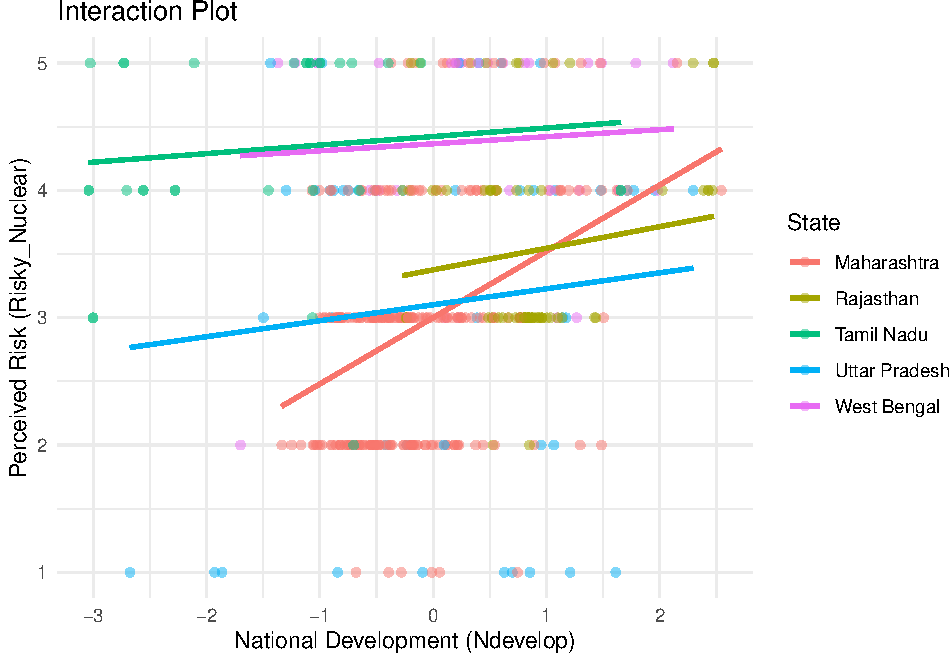
\includegraphics{Paper1_files/figure-latex/unnamed-chunk-24-1.pdf}

\begin{verbatim}
##                GVIF Df GVIF^(1/(2*Df))
## Uppercaste 1.072628  1        1.035678
## Male       1.455901  1        1.206607
## Hindu      1.097669  1        1.047697
## Urban      1.445271  1        1.202194
## age        1.127898  1        1.062026
## State      5.433827  4        1.235629
## Pdevelop   2.635311  1        1.623364
## Ndevelop   1.763451  1        1.327950
## KahanS     4.073289  1        2.018239
## KahanH     3.967258  1        1.991798
\end{verbatim}

\hypertarget{graphs-for-lm-attempts}{%
\section{graphs for lm attempts}\label{graphs-for-lm-attempts}}

\begin{Shaded}
\begin{Highlighting}[]
\FunctionTok{str}\NormalTok{(fascale\_scores) }
\end{Highlighting}
\end{Shaded}

\begin{verbatim}
## 'data.frame':    405 obs. of  48 variables:
##  $ K_IINTRFER     : num  5 2 2 5 4 1 2 1 5 5 ...
##  $ K_IPRIVACY     : num  5 4 2 1 1 4 2 1 1 5 ...
##  $ K_SHARM        : num  1 5 5 5 5 2 4 5 2 5 ...
##  $ K_IPROTECT     : num  1 2 1 5 1 2 3 1 3 5 ...
##  $ K_SLIMCHOI     : num  5 5 5 5 5 5 3 1 1 5 ...
##  $ K_SPROTECT     : num  1 4 5 5 5 5 3 5 5 5 ...
##  $ K_HEQUAL       : num  1 1 1 5 2 2 5 1 4 1 ...
##  $ K_HREVDIS1     : num  1 2 1 5 1 2 2 1 4 1 ...
##  $ K_EDISCRIM     : num  5 5 4 5 5 4 5 5 3 5 ...
##  $ K_ERADEQ1      : num  5 5 5 5 5 4 4 5 4 5 ...
##  $ K_EWEALTH      : num  5 4 5 5 5 4 4 5 5 1 ...
##  $ K_ERADEQ2      : num  5 5 4 5 5 3 5 5 2 5 ...
##  $ Risky_Nuclear  : num  4 2 5 1 4 5 4 1 2 1 ...
##  $ WEALTHLIM      : num  1 2 2 5 1 5 4 5 5 5 ...
##  $ MECHANISATION  : num  5 5 5 5 5 5 4 5 2 5 ...
##  $ DECISIONDECEN  : num  5 5 4 1 5 4 2 5 3 1 ...
##  $ DECISIONCEN    : num  1 1 2 1 1 2 3 1 2 1 ...
##  $ INDUSTRYLARGE  : num  1 1 4 1 1 2 2 1 3 1 ...
##  $ INDUSTRYSMALL  : num  5 5 5 1 5 4 4 1 3 5 ...
##  $ ECONOMYGLOBAL  : num  1 2 5 2 1 1 3 1 4 4 ...
##  $ ECONOMYLOCAL   : num  1 4 1 2 1 5 4 1 4 1 ...
##  $ ENVOVERDEV     : num  1 2 5 5 1 2 5 4 3 5 ...
##  $ DEVOVERENV     : num  4 2 1 1 1 5 3 2 3 5 ...
##  $ OWNERPVT       : num  1 4 2 4 1 1 4 5 4 5 ...
##  $ OWNERNOREG     : num  1 4 2 1 2 2 3 1 4 2 ...
##  $ OWNERPUB       : num  1 2 1 5 4 4 3 5 2 5 ...
##  $ OWNERREG       : num  5 5 4 5 5 5 3 4 5 5 ...
##  $ DISPLACENUCLEAR: num  4 1 5 1 3 4 4 5 1 1 ...
##  $ POLLUTENUCLEAR : num  5 2 5 5 5 2 4 5 4 5 ...
##  $ HEALTHNUCLEAR  : num  5 1 5 5 4 5 5 5 2 5 ...
##  $ JOBSNUCLEAR    : num  4 1 5 1 4 2 3 1 4 1 ...
##  $ BEAUTYNUCLEAR  : num  5 2 5 5 3 5 4 5 3 5 ...
##  $ PRIDENUCLEAR   : num  4 1 2 5 4 2 3 1 5 1 ...
##  $ NPRIDENUCLEAR  : num  5 1 2 4 5 1 3 5 3 1 ...
##  $ DEVNUCLEAR     : num  5 1 2 4 5 4 3 5 5 1 ...
##  $ PROSPERNUCLEAR : num  5 4 4 1 5 2 3 1 5 1 ...
##  $ RELYNUCLEAR    : num  4 1 1 5 5 5 4 1 3 1 ...
##  $ Uppercaste     : num  0 0 0 0 0 0 1 0 0 0 ...
##  $ Male           : num  0 1 1 1 1 1 1 1 1 1 ...
##  $ Hindu          : num  1 1 0 1 1 1 0 1 1 1 ...
##  $ urban_rural    : chr  "Rural" "Rural" "Rural" "Rural" ...
##  $ Urban          : Factor w/ 2 levels "Rural","Urban": 1 1 1 1 1 1 1 1 1 1 ...
##  $ State          : Factor w/ 5 levels "Maharashtra",..: 4 5 5 4 4 5 5 4 4 4 ...
##  $ age            : num  3 3 4 2 2 1 5 3 3 1 ...
##  $ KahanS         : num  -0.0649 1.4437 1.5366 1.4377 1.6015 ...
##  $ KahanH         : num  -0.952 -1.228 -1.09 -0.834 -1.259 ...
##  $ Pdevelop       : num  1.045 -0.282 1.577 0.517 0.552 ...
##  $ Ndevelop       : num  1.77 -1.7 -1.219 0.627 1.95 ...
\end{verbatim}

\begin{Shaded}
\begin{Highlighting}[]
\FunctionTok{ggplot}\NormalTok{(fascale\_scores, }\FunctionTok{aes}\NormalTok{(}\AttributeTok{x =}\NormalTok{ Pdevelop, }\AttributeTok{y =}\NormalTok{ Risky\_Nuclear)) }\SpecialCharTok{+}
  \FunctionTok{geom\_point}\NormalTok{() }\SpecialCharTok{+}  \CommentTok{\# or geom\_line() depending on how you want to visualize it}
  \FunctionTok{facet\_wrap}\NormalTok{(}\SpecialCharTok{\textasciitilde{}}\NormalTok{ State) }\SpecialCharTok{+}  \CommentTok{\# This will create separate plots for each State}
  \FunctionTok{labs}\NormalTok{(}\AttributeTok{title =} \StringTok{"Risky Nuclear vs Pdevelop by State"}\NormalTok{,}
       \AttributeTok{x =} \StringTok{"Pdevelop"}\NormalTok{,}
       \AttributeTok{y =} \StringTok{"Risky Nuclear"}\NormalTok{) }\SpecialCharTok{+}
  \FunctionTok{theme\_minimal}\NormalTok{()}
\end{Highlighting}
\end{Shaded}

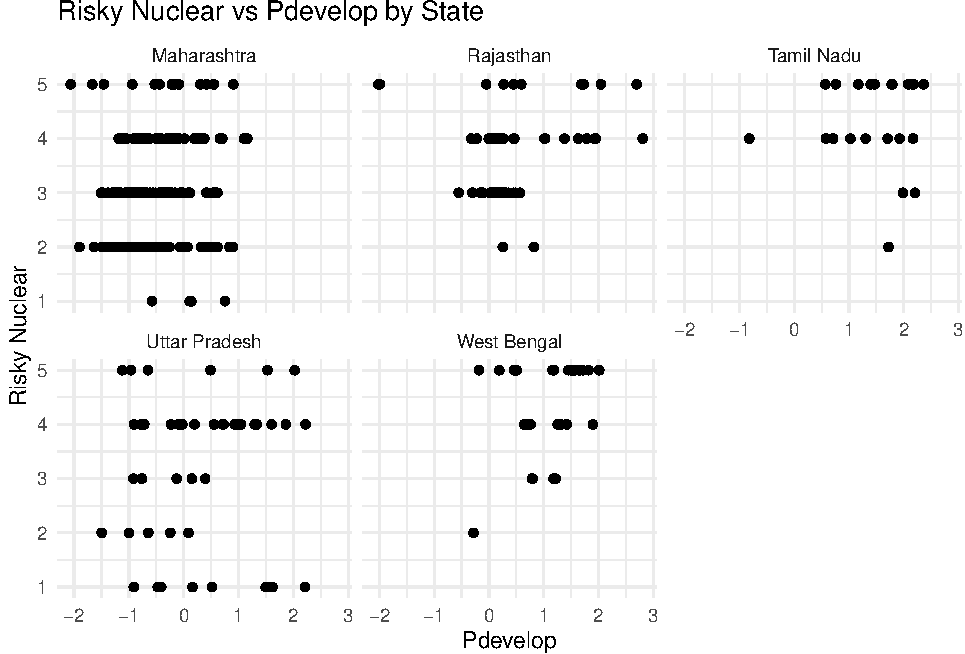
\includegraphics{Paper1_files/figure-latex/unnamed-chunk-25-1.pdf}

\begin{Shaded}
\begin{Highlighting}[]
\FunctionTok{ggplot}\NormalTok{(fascale\_scores, }\FunctionTok{aes}\NormalTok{(}\AttributeTok{x =}\NormalTok{ Ndevelop, }\AttributeTok{y =}\NormalTok{ Risky\_Nuclear)) }\SpecialCharTok{+}
  \FunctionTok{geom\_jitter}\NormalTok{(}\AttributeTok{alpha =} \FloatTok{0.5}\NormalTok{, }\AttributeTok{width =} \FloatTok{0.2}\NormalTok{) }\SpecialCharTok{+}
  \CommentTok{\#facet\_wrap(\textasciitilde{} State) +}
  \FunctionTok{geom\_smooth}\NormalTok{(}\AttributeTok{method =} \StringTok{"lm"}\NormalTok{, }\AttributeTok{se =} \ConstantTok{FALSE}\NormalTok{) }\SpecialCharTok{+}
  \FunctionTok{labs}\NormalTok{(}\AttributeTok{title =} \StringTok{"Relationship between Ndevelop and Risky Nuclear"}\NormalTok{,}
       \AttributeTok{x =} \StringTok{"Ndevelop"}\NormalTok{,}
       \AttributeTok{y =} \StringTok{"Risky Nuclear"}\NormalTok{) }\SpecialCharTok{+}
  \FunctionTok{theme\_minimal}\NormalTok{()}
\end{Highlighting}
\end{Shaded}

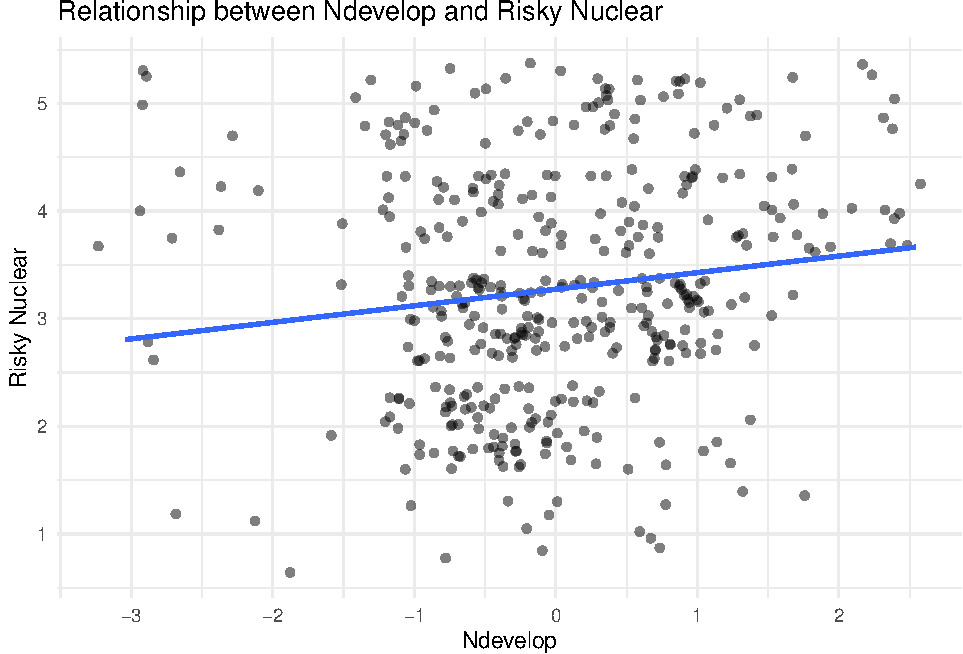
\includegraphics{Paper1_files/figure-latex/unnamed-chunk-25-2.pdf}

\begin{Shaded}
\begin{Highlighting}[]
\FunctionTok{ggplot}\NormalTok{(fascale\_scores, }\FunctionTok{aes}\NormalTok{(}\AttributeTok{x =}\NormalTok{ Pdevelop, }\AttributeTok{y =}\NormalTok{ Risky\_Nuclear)) }\SpecialCharTok{+}
  \FunctionTok{geom\_jitter}\NormalTok{(}\AttributeTok{alpha =} \FloatTok{0.5}\NormalTok{, }\AttributeTok{width =} \FloatTok{0.2}\NormalTok{) }\SpecialCharTok{+}
  \FunctionTok{facet\_wrap}\NormalTok{(}\SpecialCharTok{\textasciitilde{}}\NormalTok{ State) }\SpecialCharTok{+}
  \FunctionTok{geom\_smooth}\NormalTok{(}\AttributeTok{method =} \StringTok{"lm"}\NormalTok{, }\AttributeTok{se =} \ConstantTok{FALSE}\NormalTok{) }\SpecialCharTok{+}
  \FunctionTok{labs}\NormalTok{(}\AttributeTok{title =} \StringTok{"Relationship between Ndevelop and Risky Nuclear"}\NormalTok{,}
       \AttributeTok{x =} \StringTok{"Ndevelop"}\NormalTok{,}
       \AttributeTok{y =} \StringTok{"Risky Nuclear"}\NormalTok{) }\SpecialCharTok{+}
  \FunctionTok{theme\_minimal}\NormalTok{()}
\end{Highlighting}
\end{Shaded}

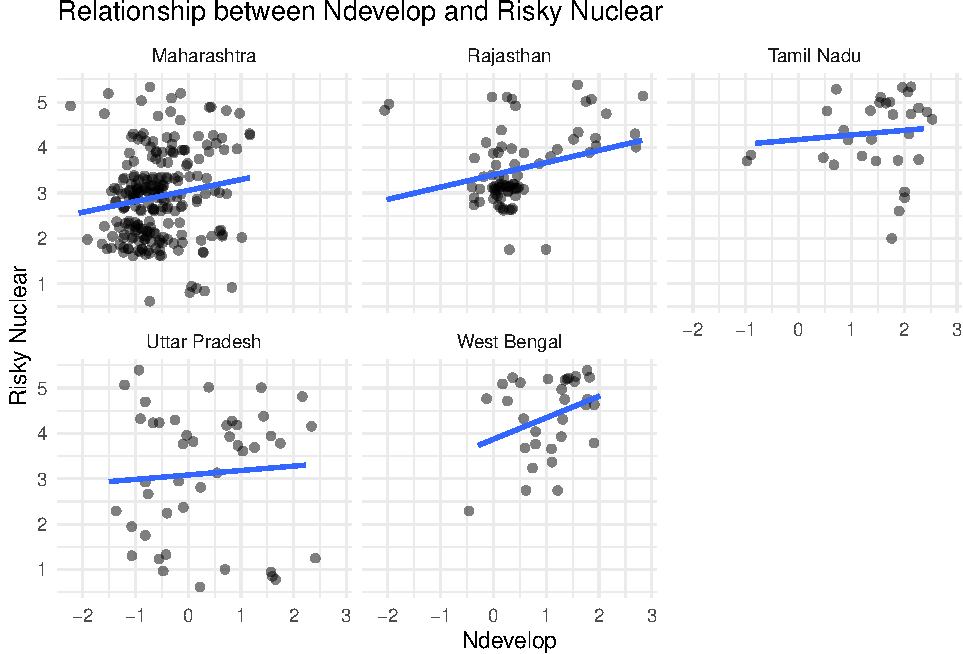
\includegraphics{Paper1_files/figure-latex/unnamed-chunk-25-3.pdf}

\begin{Shaded}
\begin{Highlighting}[]
\FunctionTok{ggplot}\NormalTok{(fascale\_scores, }\FunctionTok{aes}\NormalTok{(}\AttributeTok{x =}\NormalTok{ State, }\AttributeTok{y =}\NormalTok{ Risky\_Nuclear)) }\SpecialCharTok{+}
  \FunctionTok{geom\_boxplot}\NormalTok{() }\SpecialCharTok{+}
  \CommentTok{\#facet\_wrap(\textasciitilde{} State) +}
  \FunctionTok{theme\_minimal}\NormalTok{()}
\end{Highlighting}
\end{Shaded}

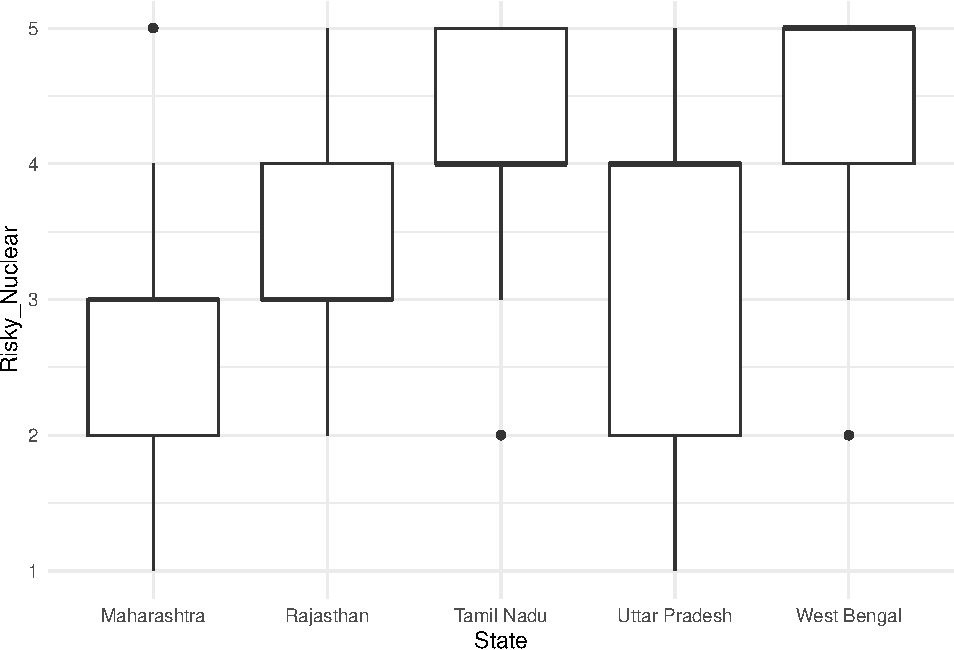
\includegraphics{Paper1_files/figure-latex/unnamed-chunk-25-4.pdf}

\newpage

\hypertarget{h4-economic-and-political-values-will-be-important-in-explaining-perceived-risk-from-nuclear-energy}{%
\section{H4 : Economic and Political Values will be important in
explaining perceived risk from Nuclear
Energy}\label{h4-economic-and-political-values-will-be-important-in-explaining-perceived-risk-from-nuclear-energy}}

\begingroup\setlength{\tabcolsep}{1pt}

\renewcommand{\arraystretch}{0.7}

\% Table created by stargazer v.5.2.3 by Marek Hlavac, Social Policy
Institute. E-mail: marek.hlavac at gmail.com \% Date and time: Sat, Jan
13, 2024 - 17:42:20

\begin{table}[!htbp] \centering 
  \caption{Results from 2 linear regression models} 
  \label{} 
\begin{tabular}{@{\extracolsep{5pt}}lcc} 
\\[-1.8ex]\hline 
\hline \\[-1.8ex] 
 & \multicolumn{2}{c}{\textit{Dependent variable:}} \\ 
\cline{2-3} 
\\[-1.8ex] & \multicolumn{2}{c}{Risky\_Nuclear} \\ 
\\[-1.8ex] & (1) & (2)\\ 
\hline \\[-1.8ex] 
 Uppercaste & $-$0.029 & $-$0.035 \\ 
  & (0.107) & (0.105) \\ 
  & & \\ 
 Male & $-$0.102 & $-$0.085 \\ 
  & (0.117) & (0.116) \\ 
  & & \\ 
 Hindu & $-$0.025 & 0.025 \\ 
  & (0.118) & (0.117) \\ 
  & & \\ 
 UrbanUrban & $-$0.003 & 0.021 \\ 
  & (0.112) & (0.111) \\ 
  & & \\ 
 age & 0.050 & 0.036 \\ 
  & (0.052) & (0.051) \\ 
  & & \\ 
 StateRajasthan & 0.445$^{***}$ & 0.186 \\ 
  & (0.169) & (0.181) \\ 
  & & \\ 
 StateTamil Nadu & 1.141$^{***}$ & 1.282$^{***}$ \\ 
  & (0.197) & (0.240) \\ 
  & & \\ 
 StateUttar Pradesh & $-$0.006 & $-$0.061 \\ 
  & (0.192) & (0.193) \\ 
  & & \\ 
 StateWest Bengal & 1.120$^{***}$ & 0.965$^{***}$ \\ 
  & (0.216) & (0.226) \\ 
  & & \\ 
 Pdevelop &  & 0.159$^{**}$ \\ 
  &  & (0.075) \\ 
  & & \\ 
 Ndevelop &  & 0.230$^{***}$ \\ 
  &  & (0.061) \\ 
  & & \\ 
 KahanS & 0.202$^{*}$ & 0.120 \\ 
  & (0.110) & (0.111) \\ 
  & & \\ 
 KahanH & $-$0.077 & 0.012 \\ 
  & (0.102) & (0.102) \\ 
  & & \\ 
 Constant & 3.008$^{***}$ & 3.033$^{***}$ \\ 
  & (0.173) & (0.172) \\ 
  & & \\ 
\hline \\[-1.8ex] 
Observations & 405 & 405 \\ 
R$^{2}$ & 0.260 & 0.290 \\ 
Adjusted R$^{2}$ & 0.240 & 0.267 \\ 
Residual Std. Error & 0.941 (df = 393) & 0.924 (df = 391) \\ 
F Statistic & 12.573$^{***}$ (df = 11; 393) & 12.298$^{***}$ (df = 13; 391) \\ 
\hline 
\hline \\[-1.8ex] 
\textit{Note:}  & \multicolumn{2}{r}{$^{*}$p$<$0.1; $^{**}$p$<$0.05; $^{***}$p$<$0.01} \\ 
\end{tabular} 
\end{table} 
\endgroup

\begingroup\setlength{\tabcolsep}{1pt}

\renewcommand{\arraystretch}{0.7}

\% Table created by stargazer v.5.2.3 by Marek Hlavac, Social Policy
Institute. E-mail: marek.hlavac at gmail.com \% Date and time: Sat, Jan
13, 2024 - 17:42:20

\begin{table}[!htbp] \centering 
  \caption{Results from 2 linear regression models} 
  \label{} 
\begin{tabular}{@{\extracolsep{5pt}}lcc} 
\\[-1.8ex]\hline 
\hline \\[-1.8ex] 
 & \multicolumn{2}{c}{\textit{Dependent variable:}} \\ 
\cline{2-3} 
\\[-1.8ex] & \multicolumn{2}{c}{Risky\_Nuclear} \\ 
\\[-1.8ex] & (1) & (2)\\ 
\hline \\[-1.8ex] 
 Uppercaste & $-$0.042 & $-$0.035 \\ 
  & (0.105) & (0.105) \\ 
  & & \\ 
 Male & $-$0.084 & $-$0.085 \\ 
  & (0.115) & (0.116) \\ 
  & & \\ 
 Hindu & 0.027 & 0.025 \\ 
  & (0.117) & (0.117) \\ 
  & & \\ 
 UrbanUrban & 0.034 & 0.021 \\ 
  & (0.110) & (0.111) \\ 
  & & \\ 
 age & 0.038 & 0.036 \\ 
  & (0.051) & (0.051) \\ 
  & & \\ 
 StateRajasthan & 0.186 & 0.186 \\ 
  & (0.180) & (0.181) \\ 
  & & \\ 
 StateTamil Nadu & 1.322$^{***}$ & 1.282$^{***}$ \\ 
  & (0.239) & (0.240) \\ 
  & & \\ 
 StateUttar Pradesh & $-$0.011 & $-$0.061 \\ 
  & (0.189) & (0.193) \\ 
  & & \\ 
 StateWest Bengal & 1.017$^{***}$ & 0.965$^{***}$ \\ 
  & (0.223) & (0.226) \\ 
  & & \\ 
 Pdevelop & 0.207$^{***}$ & 0.159$^{**}$ \\ 
  & (0.064) & (0.075) \\ 
  & & \\ 
 Ndevelop & 0.256$^{***}$ & 0.230$^{***}$ \\ 
  & (0.057) & (0.061) \\ 
  & & \\ 
 KahanS &  & 0.120 \\ 
  &  & (0.111) \\ 
  & & \\ 
 KahanH &  & 0.012 \\ 
  &  & (0.102) \\ 
  & & \\ 
 Constant & 3.011$^{***}$ & 3.033$^{***}$ \\ 
  & (0.171) & (0.172) \\ 
  & & \\ 
\hline \\[-1.8ex] 
Observations & 405 & 405 \\ 
R$^{2}$ & 0.287 & 0.290 \\ 
Adjusted R$^{2}$ & 0.267 & 0.267 \\ 
Residual Std. Error & 0.924 (df = 393) & 0.924 (df = 391) \\ 
F Statistic & 14.356$^{***}$ (df = 11; 393) & 12.298$^{***}$ (df = 13; 391) \\ 
\hline 
\hline \\[-1.8ex] 
\textit{Note:}  & \multicolumn{2}{r}{$^{*}$p$<$0.1; $^{**}$p$<$0.05; $^{***}$p$<$0.01} \\ 
\end{tabular} 
\end{table} 
\endgroup
\newpage

\hypertarget{logistic-regression}{%
\section{Logistic Regression}\label{logistic-regression}}

\begin{table}[!h]

\caption{\label{tab:unnamed-chunk-28}Odds Ratio for Perceived Risk from Nuclear Energy}
\centering
\begin{tabular}[t]{lrrrr}
\toprule
  & Odds Ratio & 2.5 \% & 97.5 \% & p value\\
\midrule
\cellcolor{gray!6}{Uppercaste} & \cellcolor{gray!6}{-0.151} & \cellcolor{gray!6}{-0.561} & \cellcolor{gray!6}{0.258} & \cellcolor{gray!6}{0.469}\\
Male & -0.179 & -0.627 & 0.267 & 0.432\\
\cellcolor{gray!6}{Hindu} & \cellcolor{gray!6}{0.008} & \cellcolor{gray!6}{-0.449} & \cellcolor{gray!6}{0.466} & \cellcolor{gray!6}{0.971}\\
UrbanUrban & 0.036 & -0.397 & 0.469 & 0.870\\
\cellcolor{gray!6}{age} & \cellcolor{gray!6}{0.082} & \cellcolor{gray!6}{-0.121} & \cellcolor{gray!6}{0.287} & \cellcolor{gray!6}{0.429}\\
\addlinespace
KahanS & 0.276 & -0.188 & 0.738 & 0.243\\
\cellcolor{gray!6}{KahanH} & \cellcolor{gray!6}{0.063} & \cellcolor{gray!6}{-0.351} & \cellcolor{gray!6}{0.477} & \cellcolor{gray!6}{0.765}\\
Pdevelop & 0.445 & 0.123 & 0.770 & 0.007\\
\cellcolor{gray!6}{Ndevelop} & \cellcolor{gray!6}{0.447} & \cellcolor{gray!6}{0.186} & \cellcolor{gray!6}{0.712} & \cellcolor{gray!6}{0.001}\\
StateRajasthan & 0.164 & -0.554 & 0.883 & 0.655\\
\addlinespace
\cellcolor{gray!6}{StateTamil Nadu} & \cellcolor{gray!6}{2.538} & \cellcolor{gray!6}{1.508} & \cellcolor{gray!6}{3.605} & \cellcolor{gray!6}{0.000}\\
StateUttar Pradesh & -0.003 & -0.834 & 0.822 & 0.994\\
\cellcolor{gray!6}{StateWest Bengal} & \cellcolor{gray!6}{1.947} & \cellcolor{gray!6}{0.999} & \cellcolor{gray!6}{2.924} & \cellcolor{gray!6}{0.000}\\
\bottomrule
\end{tabular}
\end{table}

\newpage

\hypertarget{appendix-characteristics-of-the-sample}{%
\section{Appendix: Characteristics of the
Sample}\label{appendix-characteristics-of-the-sample}}

The following graph shows that distribution of different demographic
variables in our sample of 2,160 from the combined dataset from both
surveys. The percentages are rounded off to whole numbers.

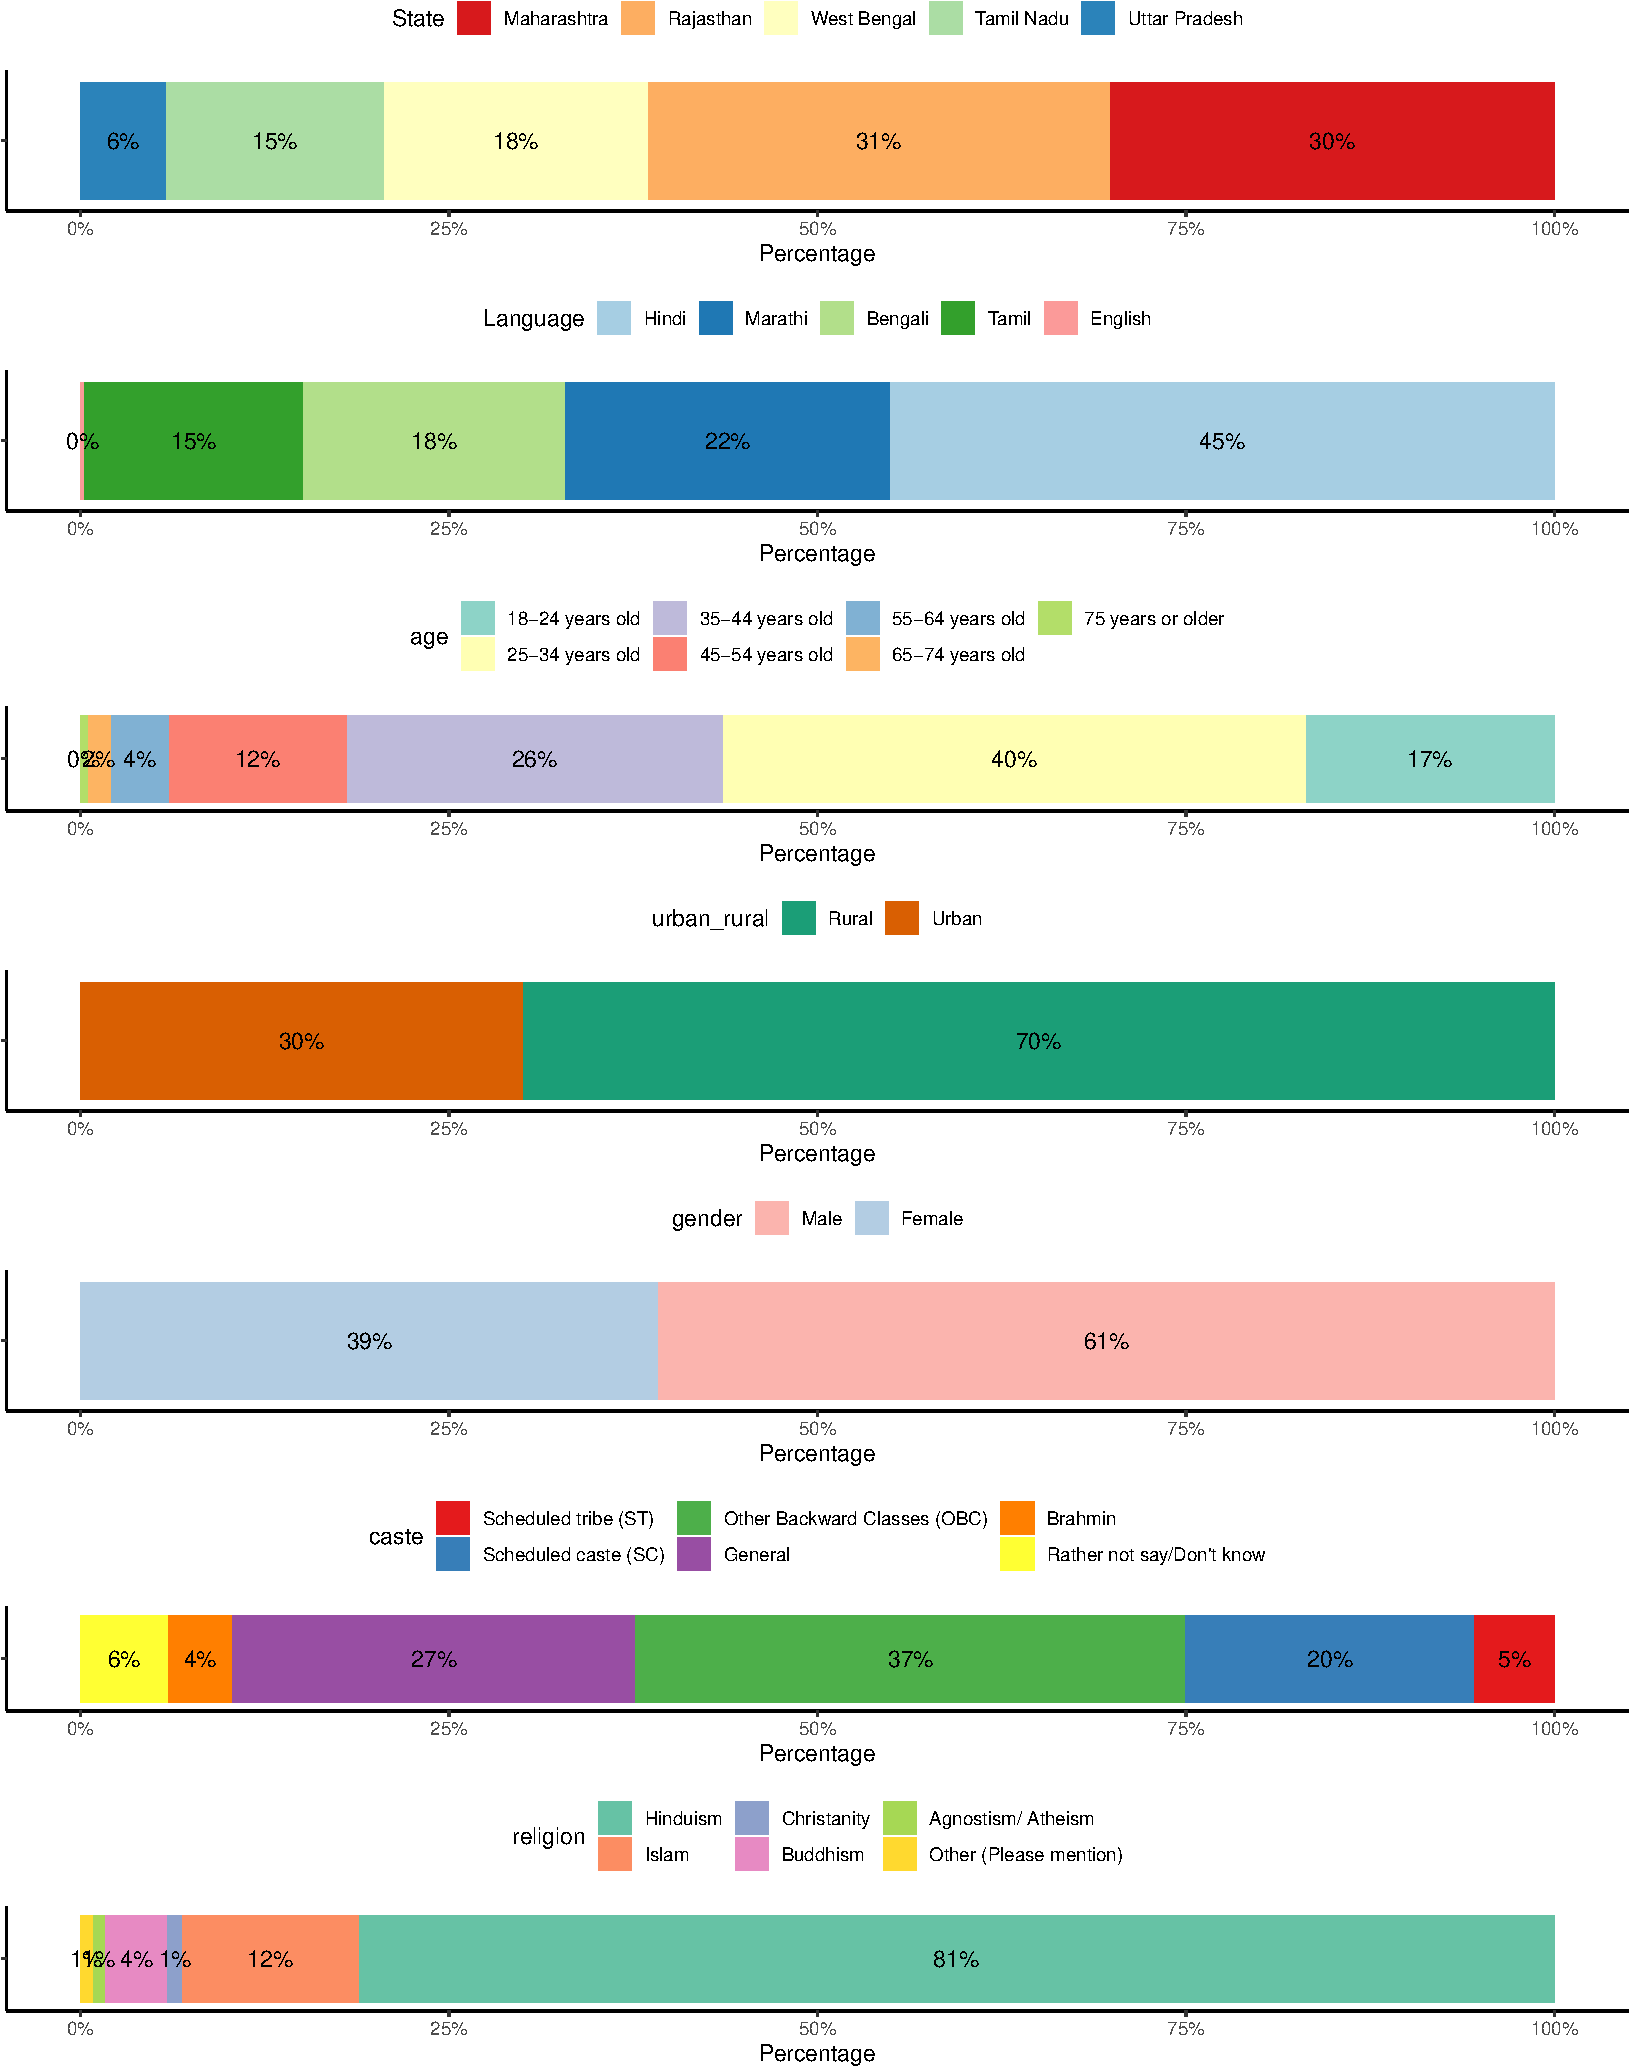
\includegraphics[width=0.8\linewidth,height=0.8\textheight]{Paper1_files/figure-latex/unnamed-chunk-32-1}

\end{document}
